% =====2-review outline======
% 1. intro 文献综述部分:重写、补充,引用c8的文献;对RBS性能的分析
%   1.1 任务分配:如果从电流分配的角度考虑,这是一个 NP-hard 问题,求解这类问题的开销一般很大,通过针对性地改进传统算法来解决计算开销,例如 Mollajafari 提出了 a meta-heuristic method named Graph-Oriented Simulated Annealing (GOSA) )(结合 gammoudiEnergyEfficientSchedulingRealTime2020 这篇可重构任务调度的文章)
%   1.2 对RBS性能的分析
%   1.3 多说一点启发式算法
% 2. case study 增加实验 模拟退火、遗传算法;增加b结构的2,6数量的电池
%   2.1 structures and details
%       2.1.1 4-battery 不同结构(3个tab:our method;1个图)
%       2.1.2 2/4/6-battery 结构c
%       2.1.3 4-battery 不同结构 isolated battery
%       2.1.4 四种计算方法
%   2.2 result: 删去table4和前面一段话;添加文字,描述figure7;使用子图子表格
%       2.1.1 c结构的计算细节:1组fig(有向图、SP、最终结果)
%       2.1.2 4-battery 不同结构的计算结果:1组tab(各结构计算结果)、2组fig(各结构MAC正确闭合方案+算法迭代过程中的MAC折线图)
%       2.1.3 2/4/6-battery 结构c(1,2,3 *2)的计算结果:1组tab(各结构计算结果)、2组fig(各结构MAC正确闭合方案+算法迭代过程中的MAC折线图)
%       2.1.4 4-battery c 不同 isolated battery 的计算结果:1组fig(不同电池数的开关闭合方案)
%   2.3 discussion:
%       2.3.1 结果正确性和准确性:a. 电路分析;b. 与 force-brute 结果的验证
%       2.3.2 算法的有效性和优劣:a. 复杂度;b. 与 SA、GA 的比较(启发式算法仅找到局部最优;收敛时间);c. 本算法的优劣和原因
%       2.3.3 this work 的意义和应用:a. 说明 eta 的意义、应用方法;b. 结合 isolated battery 说明应用场景
% 3. conclusion 相关内容修改
% 4. abstract 相关内容修改

% ! NOTE
% [DONE]
% 1. red mark -> blue mark
% 2. check ref
% 3. rewrite the last two paragraphs of the introduction if time permits

\documentclass{article}
\usepackage[utf8]{inputenc}
\usepackage{authblk}
\usepackage{setspace}
\usepackage[margin=1.25in]{geometry}
\usepackage{graphicx}
% \graphicspath{ {./figures/} }
% \graphicspath{ {../figures/} }
\graphicspath{ {../../attachments} }
\usepackage{subcaption}
\usepackage{amsmath}
\usepackage{lineno}
\linenumbers

\usepackage{enumerate}
\DeclareMathOperator{\diag}{diag}
\usepackage{multirow}
\usepackage{booktabs}
\usepackage{footnote}
\usepackage{bm}
\usepackage[ruled,linesnumbered]{algorithm2e}
\setcounter{MaxMatrixCols}{20}
\usepackage{tikz}
\usetikzlibrary{arrows.meta, calc, fit, positioning, quotes, graphs, shapes.geometric}
\def\T{\mathrm{T}}

%%%%%% Bibliography %%%%%%
% Replace "sample" in the \addbibresource line below with the name of your .bib file.
% \usepackage[style=nejm, 
% citestyle=numeric-comp, 
% sorting=none]{biblatex}
% \addbibresource{ref.bib}

%%%%%% Title %%%%%%
% Full titles can be a maximum of 100 characters, including spaces. 
% Title Format: Use title case, capitalizing the first letter of each word, except for certain small words, such as articles and short prepositions
% \title{Using a Directed Graph Model and Greedy Algorithm to Determine the Maximum Allowable Current in a Reconfigurable Battery System}
\title{Maximum Allowable Current Determination of RBS By Using a Directed Graph Model and Greedy Algorithm}

%%%%%% Authors %%%%%%
% Authors should be listed in order of contribution to the paper, by first name, then middle initial (if any), followed by last name.
% Authors should be listed in the order in which they will appear in the published version if the manuscript is accepted. 
% Use an asterisk (*) to identify the corresponding author, and be sure to include that person’s e-mail address. Use symbols (in this order: †, ‡, §, ||, ¶, #, ††, ‡‡, etc.) for author notes, such as present addresses, “These authors contributed equally to this work” notations, and similar information.
% You can include group authors, but please include a list of the actual authors (the group members) in the Supplementary Materials.
\author[1$\dag$]{Binghui Xu}
\author[1$\dag$]{Guangbin Hua}
\author[1*]{Cheng Qian}
\author[1,2]{Quan Xia}
\author[1]{Bo Sun}
\author[1]{Yi Ren}
\author[1]{Zili Wang}

%%%%%% Affiliations %%%%%%
\affil[1]{School of Reliability and Systems Engineering, Beihang University, Beijing, 100191, China}
\affil[2]{School of Aeronautic Science and Engineering at Beihang University, Beijing, China}
\affil[*]{Address correspondence to: cqian@buaa.edu.cn}
\affil[$\dag$]{These authors contributed equally to this work.}

%%%%%% Date %%%%%%
% Date is optional
\date{}

%%%%%% Spacing %%%%%%
% Use paragraph spacing of 1.5 or 2 (for double spacing, use command \doublespacing)
\onehalfspacing

\begin{document}

\maketitle

%%%%%% Abstract %%%%%%
\begin{abstract}
Reconfigurable battery systems (RBSs) present a promising alternative to traditional battery systems due to their flexible and dynamically changeable topological structure that can be adapted to different battery charging and discharging strategies.
During RBS operation, a critical system parameter known as the maximum allowable current (MAC) become pivotal. This parameter is instrumental in maintaining the current of each individual battery within a safe range and serves as a guiding indicator for the system's reconfiguration, thereby ensuring its safety and reliability.
This paper proposes a method to calculate the MAC of arbitrary RBSs using a greedy algorithm in conjunction with a directed graph model of the RBS.
By introducing the shortest path (SP) of the battery, the greedy algorithm transforms the enumeration of switch states in the brute-force algorithm or variable search without utilizing structures in the heuristic algorithms (simulated annealing and genetic algorithm) into the combination of the shortest paths.
This significantly enhances the efficiency with which the MAC is determined.
The directed graph model, based on the equivalent circuit, provides a specific method for calculating the MAC of a given structure.
The proposed method is validated on two published RBS structures and one with a more complex structure.
The results are the same as those of the brute-force algorithm, but the proposed method significantly improves the computational efficiency ($N_s 2^{N_s - N_b} \log_{10} N_b$ times faster than the brute-force algorithm for an RBS with $N_b$ batteries and $N_s$ switches, theoretically).
Another advantage of the proposed method is its ability to calculate the MAC of RBSs with arbitrary structures and variable battries, even in scenarios with random isolated batteries.
\end{abstract}

\section{Introduction}

Battery energy storage systems (BESSs) are widely utilized in various applications \cite{yangBatteryEnergyStorage2018}, such as wind power plants \cite{desiqueiraControlStrategySmooth2021} and space power systems \cite{schwanbeckInternationalSpaceStation2019,zhangDevelopmentProspectChinese2021}, for the purpose of storing and releasing high-quality electrical energy \cite{choCommercialResearchBattery2015}.
Typically, a BESS consists of numerous batteries interconnected by series-parallel circuitry to provide the required storage capacity.
However, conventional BESSs, in which the batteries are connected in a fixed topology, suffer from a significant weakness in their worst battery due to the so-called cask effect.
Furthermore, if the worst battery fails during operation, it is highly likely to accelerate the degradation of the other batteries, resulting in reliability and safety issues at the system level \cite{yangUnbalancedDischargingAging2016,fengPropagationMechanismsDiagnosis2019,jeevarajanBatterySafetyQualifications2012}.
These challenges have become major technical obstacles in many engineering projects that demand high reliability, such as the development of next-generation space vehicles \cite{pomboHybridPowerSystem2021}.
Reconfigurable battery systems (RBSs), which can dynamically switch between different circuit topologies as needed, are expected to address these issues \cite{hanNextGenerationBatteryManagement2020a}.
In a typical RBS, additional switches are introduced between the batteries to form a reconfigurable network, where the circuit's topology can be altered by opening or closing the switches.
By opening the switches adjacent to the unhealthy batteries, they can be isolated from the system, ensuring that the system remains in a reliable operational state \cite{ci2016reconfigurable}.
Furthermore, the RBS can be reconfigured to adapt to different charging and discharging strategies, thereby enhancing the system's efficiency and prolonging the battery's lifespan \cite{bouchhima2018lifetime}.
These advantages make RBSs a promising alternative to traditional BESSs.


The early research on RBSs mainly focused on the topological design of the structure, incorporating different levels of flexibility and reconfigurability to meet application requirements.
For example, Ci et al. \cite{ci2007novel} proposed an RBS structure that dynamically adjusts the battery discharge rate to fully exploit the available capacity of each battery. 
Jan's \cite{9209774,engelhardt2021double} structures reconfigure circuits with variant batteries in series to accommodate the constantly changing voltage requirements during electric vehicle charging.
The structure proposed by Visairo et al. \cite{visairoReconfigurableBatteryPack2008} alters the system's output voltage based on the load conditions, thereby reducing power loss in the voltage regulator during the power supply process and enhancing energy efficiency. 
Also, to enhance the energy efficiency of the system, Lawson et al. \cite{lawsonSoftwareConfigurableBattery2012} and He et al. \cite{he2014reconfiguration}  proposed simplified structures that have fewer switches than Visairo's design.
Kim et al. \cite{kim2009dynamic} improved the system's ability to recover from battery failures by introducing multiple ports into the structure. 
However, these complex structures between batteries and switches provide flexibility to RBSs while also posing challenges in hardware design. 
During the reconfiguration process, current deviation and fluctuation may occur. Specifically, when the system switches from series to parallel connection, circulating current between parallel cells can be triggered due to voltage imbalance \cite{hanAnalysisEstimationMaximum2020}. Failure to fully consider this issue during the design of RBSs can result in damage to the batteries, switches, and wires. 
For example, Engelhardt et al. \cite{engelhardtDoubleStringBatterySystem2021} applied RBS to a fast-charging scenario with adaptive cell switching, which can balance cell states while adhering to voltage requests. However, the switching of batteries leads to intolerable current variations. 
To address this problem, Han et al. \cite{han2021analysis} derived an analytical expression for the maximum switch current during battery system reconfiguration. This analytical expression aids in the selection of switches and supports the hardware design of RBSs.


Recently, there has been increasing attention given to the estimation and control of the system state of RBSs, and several approaches have been proposed to optimize the performance of the system. 
State estimation, which is an essential technology in traditional battery management systems, serves as the foundation for system control and holds great potential in the context of RBSs \cite{komsiyskaCriticalReviewIntelligent2021}.
Couto et al. \cite{coutoPartitionbasedUnscentedKalman2018a} introduced a partition-based unscented Kalman filter to estimate the state of a large-scale RBS, utilizing an enhanced reduced-order electrochemical model. 
Kersten et al. \cite{kerstenOnlineOnBoardBattery2020a} utilized the balancing current of neighboring cells in parallel operation to determine battery impedances, thereby obtaining information about the state of health and power capability. 
Schmid et al. \cite{schmidActiveModelBasedFault2021a} further leveraged the reconfigurable nature of the system to actively diagnose faults, employing an algorithm that changes the system structure to enhance fault isolability. 
Another active research topic is the development of effective control strategies for RBSs to achieve optimal performance, including improved stability \cite{kacetlDesignAnalysisModular2023b} and efficiency \cite{yangAdaptiveControlFramework2022}.
Han et al. \cite{hanNearFastestBatteryBalancing2019a} proposed a near-fastest battery balancing algorithm to minimize the time required for battery charge equalization.
Liu et al. \cite{liuFlexiblePathPlanningbased2023a} also proposed a scheme for maximizing capacity utilization based on a path planning algorithm, aiming to enhance battery consistency within the system.
To break through the bootleneck of the potential short-circuit paths increase exponentially with the RBS's scale, Chen et al. \cite{chenSneakCircuitTheory2021} proposed a systematic approach based on sneak circuit theory. 
They conducted a comprehensive analysis of all paths between the cathode and anode of each battery in the RBS, identifying paths that only consist of switches as short-circuit paths for pre-checking before system reconfiguration. 
Furthermore, Artificial Intelligence also appears in the RBS management \cite{liuLongLifetimeBattery2022a}.
The effectiveness of deep reinforcement learning method has been validated in real-world RBSs \cite{yangAdaptiveControlFramework2022}.


The maximum allowable current (MAC), which is defined as the maximum current allowed within the constraints of the battery cell, is a crucial indicator of RBSs that needs to be evaluated during the design and control of the system. 
The MAC assists designers in assessing whether the RBS meets the requirements for output current and contributes to the development of appropriate and safe management strategies for the battery management system. 
Unfortunately, there have been few studies proposed to directly determine the MAC of RBSs, primarily due to the complexity arising from reconfiguration. 
In the field of computer science, there is a similar problem of scheduling tasks on dynamically reconfigurable hardware with limited resources and task interdependencies, which is analogous to the determination of MAC. 
A corresponding method has been proposed \cite{mollajafariEfficientLightweightAlgorithm2023,heReconfigurationassistedChargingLargescale2014}. 
However, dealing with the structural characteristics and circuit equations of RBSs is challenging for this method.  
From the perspective of RBS structure analysis, the MAC problem can be transformed into finding the maximum output current among all possible reconfigurations of the RBS. 
However, this may be an NP-hard problem \cite{pinterReviewControlAlgorithms2021a}. 
Common methods such as brute-force algorithms, simulated annealing (SA) algorithms, and genetic algorithms (GA) have the drawbacks of inefficiency, time consumption, and inability to guarantee the globally optimal solution.


To solve this issue, this paper proposes an efficient method to evaluate the MAC of RBSs. 
In this method, a greedy algorithm is designed to efficiently search the possible circuit topology of RBSs with MAC.
This algorithm transforms the inefficiently searching reconfigurations into the proactively combining of the shortest paths of batteries.
Furthermore, an improved directed graph model is introduced to analyze the current of the RBS, taking into account factors such as voltage, internal resistance, MAC of the battery, and external load. 
The main contributions of this study can be summarized as follows:
\begin{itemize}
  \item An efficient method is proposed to determine the MAC of RBSs with arbitrary structures, including scenarios with isolated batteries.
  \item A greedy algorithm is applied to solve the MAC problem, the computational complexity of which is greatly reduced compared with the brute-force algorithm.
  \item An improved directed graph model is introduced to provide a specific method for calculating the MAC of a given structure.
\end{itemize}


The remainder of this paper is organized as follows: 
Section II presents the framework and details of the proposed directed graph model and greedy algorithm. 
Section III examines a case study that applies the proposed method to determine the MACs of two published RBS structures and one with a more complex structure. 
The calculation results, the computational complexity of the algorithm, and scenarios such as battery random isolation are also discussed. 
Finally, the concluding remarks are presented in Section IV.

\section{Methodology}

The central principle of this method is to connect the batteries in an RBS in parallel to the extent possible, thereby maximizing the output current of the RBS.
To achieve this universally and automatically, the overall process is divided into the four steps shown in Fig. \ref{fig:main}.
First, a directed graph model is established for subsequent computations. The model not only contains the connected relationships between batteries and switches but also retains the performance parameters of the batteries.
Subsequently, based on the equivalent circuit, the MAC problem is transformed into specific objective functions and constraints.
The shortest paths (SPs, where additional batteries and switches on the path are penalized as distance) for the batteries are then obtained  by using the Dijkstra algorithm to connect the batteries in the RBS in parallel.
Finally, a greedy algorithm is used to organize the switches, allowing the batteries to connect via their SPs while satisfying the constraints, resulting in the MAC of the RBS.

\begin{figure}[htbp]
    \centering
    \begin{subfigure}[b]{0.8\textwidth}
        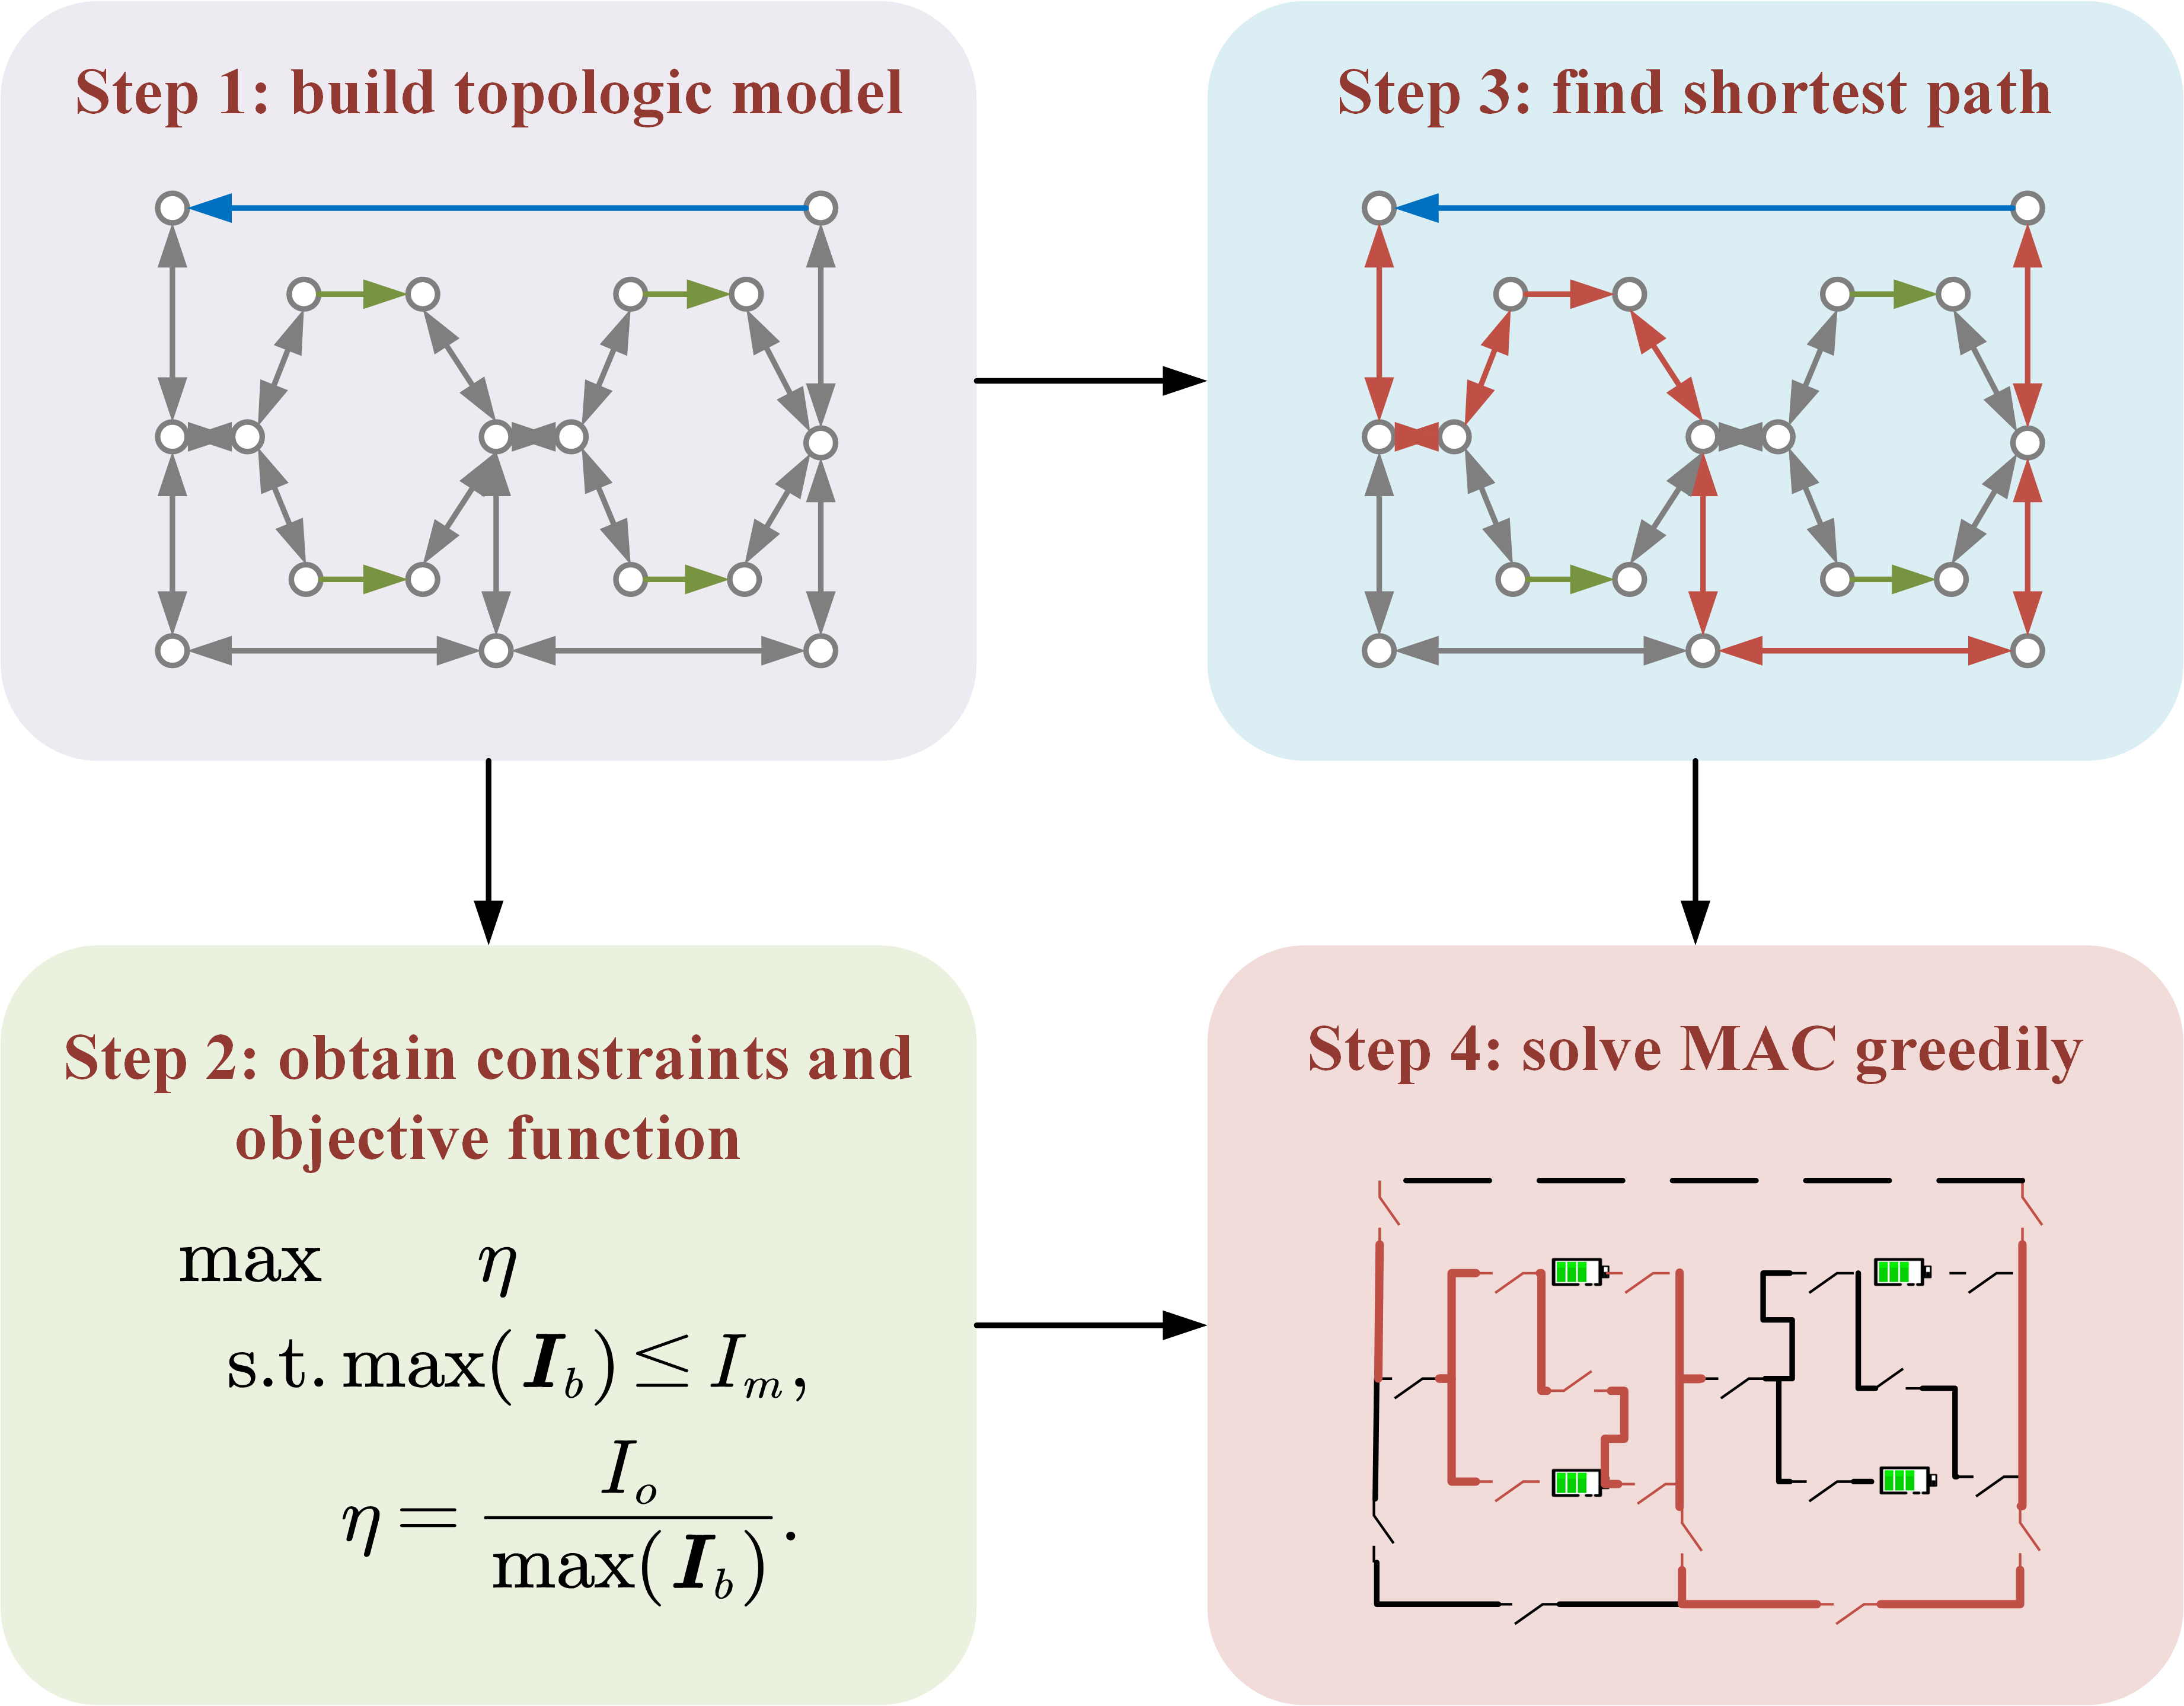
\includegraphics[width=\textwidth]{main.png}
    \end{subfigure}
    \caption{ 
        Diagram of this method, which contains four main steps.
    }
    \label{fig:main}
\end{figure}

\subsection{Directed graph model}

\begin{figure}[htbp]
    \centering
    \begin{subfigure}[b]{0.31\textwidth}
        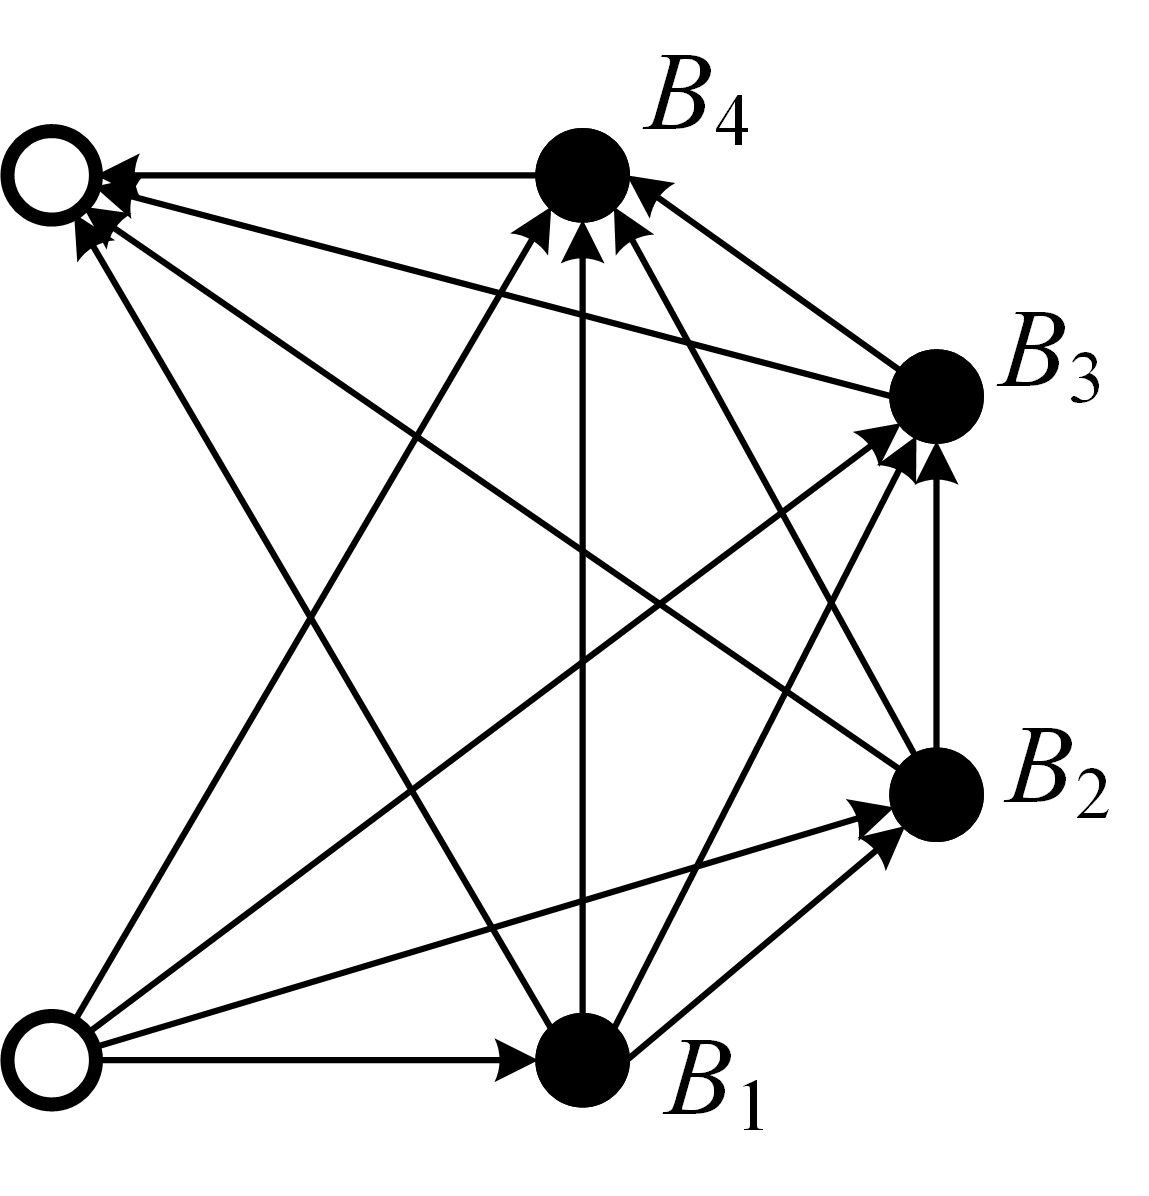
\includegraphics[width=\textwidth]{direct-graph-he.png}
        \caption{}
        \label{fig:direct-graph-he}
    \end{subfigure}
    \hspace{0.02\textwidth}
    \begin{subfigure}[b]{0.23\textwidth}
        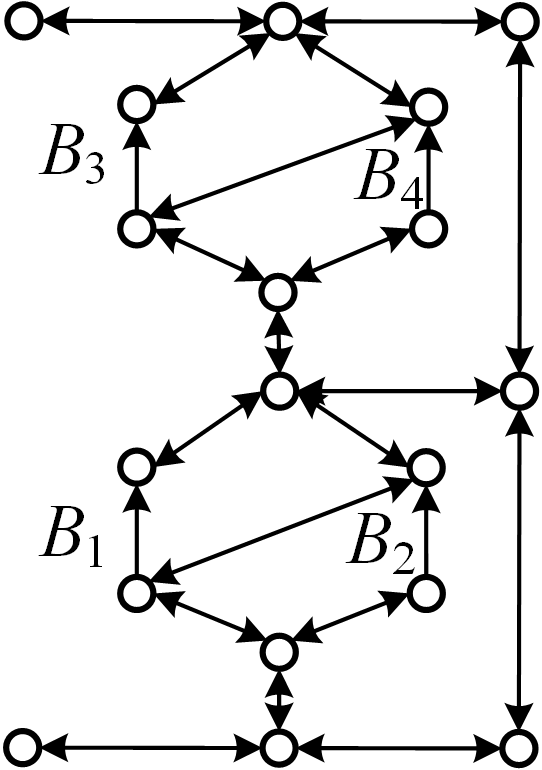
\includegraphics[width=\textwidth]{direct-graph-xu.png}
        \caption{}
        \label{fig:direct-graph-xu}
    \end{subfigure}
    \hspace{0.02\textwidth}
    \begin{subfigure}[b]{0.24\textwidth}
        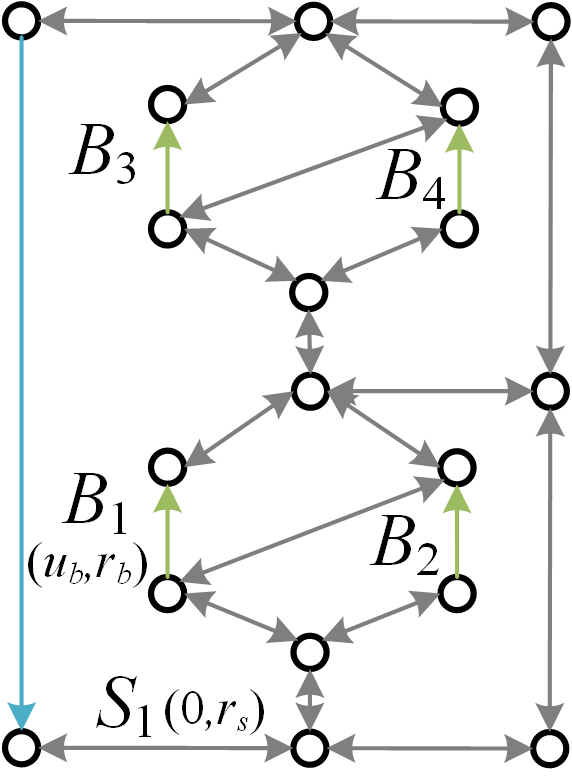
\includegraphics[width=\textwidth]{direct-graph-my.png}
        \caption{}
        \label{fig:direct-graph-my}
    \end{subfigure}
    \\
    \begin{subfigure}[b]{0.8\textwidth}
        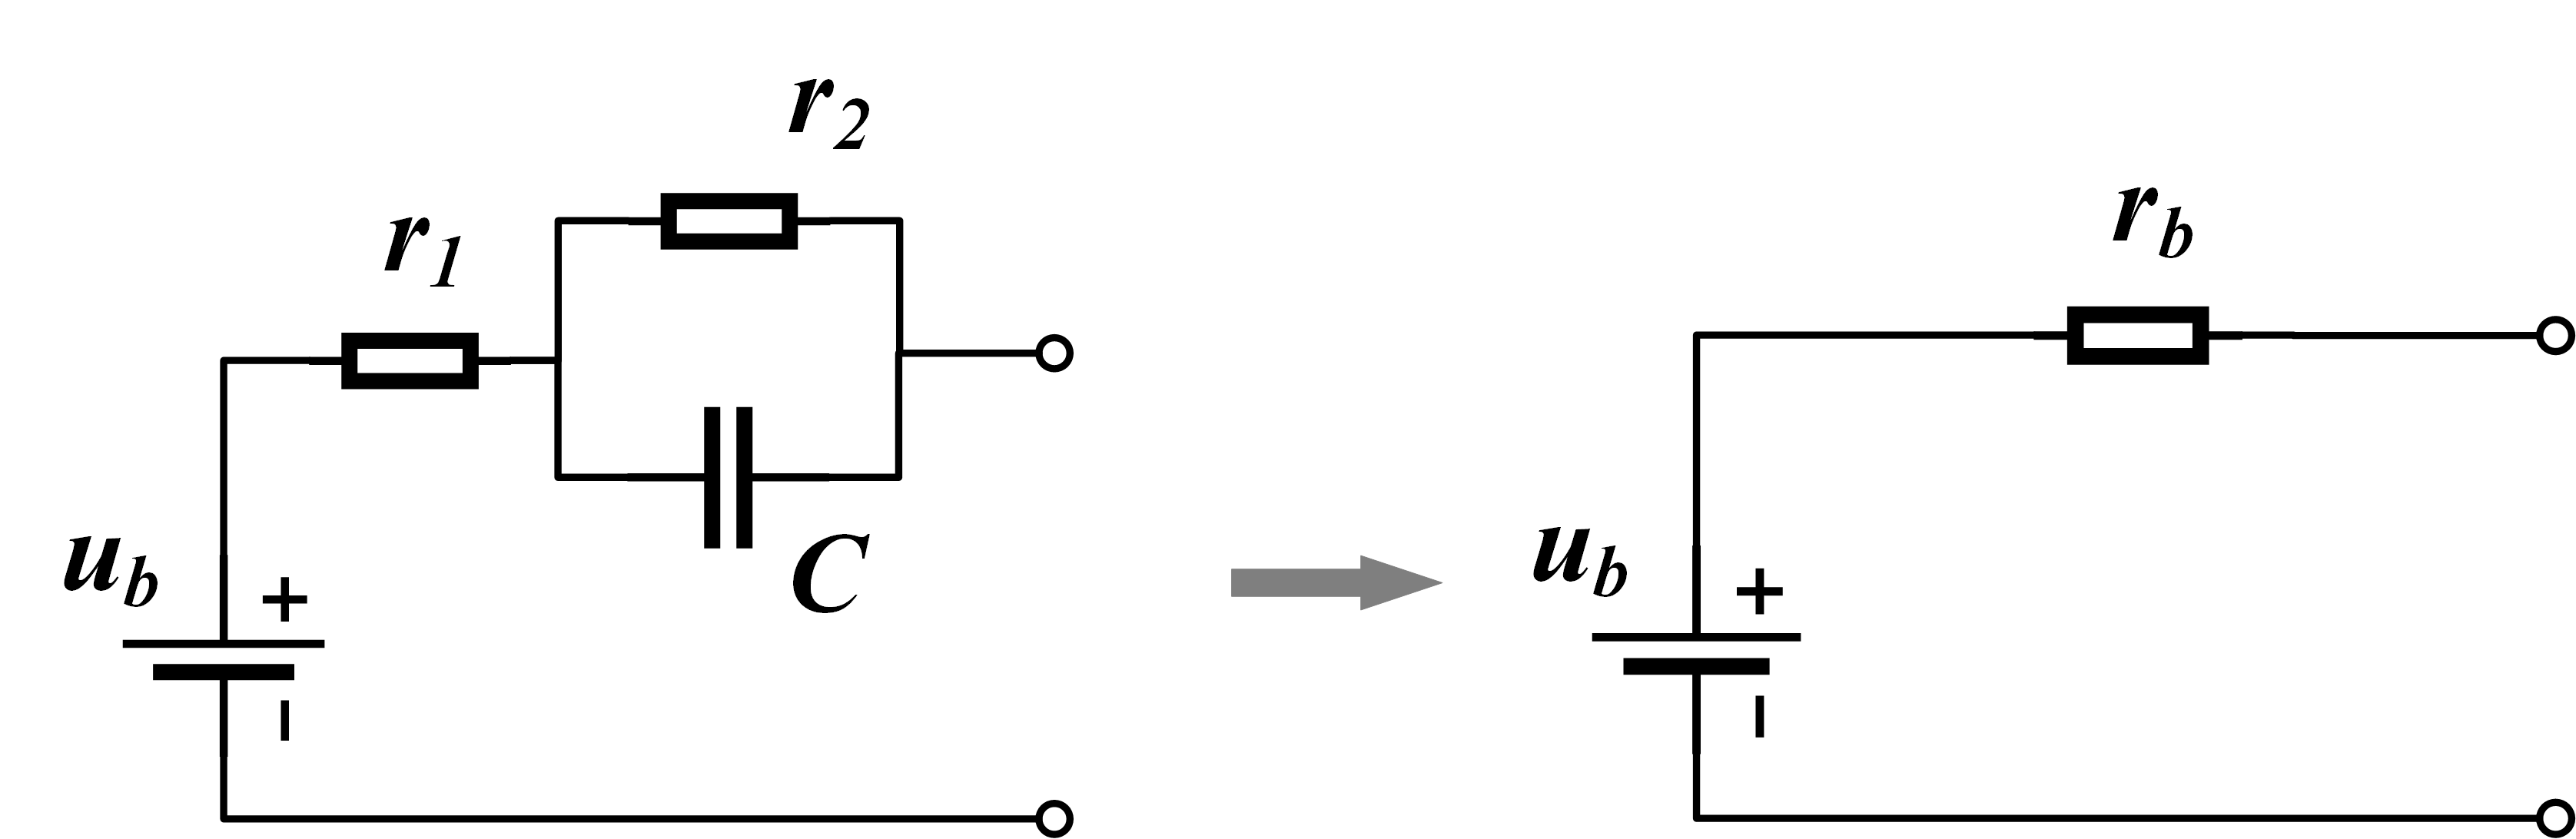
\includegraphics[width=\textwidth]{battery_simple.png}
        \caption{}
        \label{fig:battery_simple}
    \end{subfigure}
    \caption{ 
        Directed graph models used in (a) He's work \cite{heExploringAdaptiveReconfiguration2013}, (b) our previous work, and (c) the improved model in this paper.
        (d) The equivalent circuit of a battery in this method.
    }
\end{figure}

He et al. \cite{heExploringAdaptiveReconfiguration2013} proposed an abstracted directed graph model for an RBS, where the nodes represent the batteries, the edges represent the configuration flexibility, and the weight of each vertex corresponds to the battery voltage (Fig. \ref{fig:direct-graph-he}). 
The model captures all potential system configurations and offers a direct metric for configuration flexibility, but it does not specify the physical implementation of the connectivity between batteries, meaning that one graph might correspond to multiple RBS structures.
We previously proposed a directed graph model that differs completely from He's model by using nodes to represent the connections between batteries and switches and directed edges to represent batteries and switches (Fig. \ref{fig:direct-graph-xu}), allowing for a one-to-one correspondence between the RBS structure and the directed graph model. 
This model accurately and comprehensively represents the RBS topological structure but cannot be used for quantitative MAC calculations because it does not consider  the voltage, internal resistance, and MAC of the battery. 
To address this issue, we improve our previous model by adding electromotive force and resistance attributes on the edges based on its equivalent circuits.
The model also considers the external load as an equivalent resistance and integrates it into the analysis, making it a complete circuit model for later circuit analyses.
Fig. \ref{fig:direct-graph-my} shows the improved directed graph model used in this paper.
The following  provides a detailed explanation of the method for equating components in RBSs and constructing the directed graph model.


To use circuit analysis methods to solve the MAC of the RBS, the components in the RBS are equated to ideal circuit elements.
For instance, as shown in Fig. \ref{fig:battery_simple}, the battery in the RBS is represented as a black-box circuit consisting of two resistors $r_1$ and $r_2$ and a capacitor $C$, known as the Thevenin model \cite{hongwenheStateofChargeEstimationLithiumIon2011,mousavig.VariousBatteryModels2014}.
With an emphasis on the stable output of the RBS, the capacitor in the Thevenin model can be considered as an open circuit without affecting the steady-state current.
Therefore,  battery $B_i$ in the RBS can be simplified as a series connection between a constant voltage source $u_{i}$ and a resistor $r_{i}$.
Furthermore, the state of switch $S_j$ in the RBS is represented by a binary variable $x_j$, where 0 is ON and 1 is OFF.
When the switch is closed, the circuit can be regarded as a resistor with a very small resistance $r_{j}$.
Finally, the external load is considered as a resistor with resistance $R_o$.


For a given RBS structure, its directed graph model $G(V,E)$ is constructed as follows:
\begin{enumerate}
    \item Nodes:
        The nodes in the directed graph correspond to the connection points of components in the actual RBS. 
        Assuming there are a total of $N$ nodes in the RBS, for the sake of convenience, the anode of the RBS is denoted as $v_1$ and the cathode as $v_N$.
    \item Edges:
        The edges in the directed graph correspond to the batteries, switches, and external electrical loads in the actual RBS.
        Therefore, there are three types of directed edges. 
        For battery $B_i$, its directed edge $e_i$ is drawn from the cathode to the anode because the battery in operation only allows current to flow in one direction.
        For switch $S_j$, since it is allowed to work under bidirectional currents, it is represented by a pair of directed edges with two-way directions. 
        Regarding the external electronic load, because it is connected to the anode and cathode of the RBS, a directed edge from $v_N$ to $v_1$  represents it. 
        In conclusion, for a given RBS structure with $N_b$ batteries and $N_s$ switches, the number of directed edges is $N_b+2N_s+1$, where 1 refers to the external electrical load.
    \item Attributes of edges:
        Each edge is assigned two attributes, voltage difference and resistance, based on the equivalent method mentioned above.
        The values for  battery $B_i$, switch $S_j$, and external loads correspond to $(u_i, r_i)$, $(0, r_j)$, and $(0, R_o)$, respectively.
\end{enumerate}

\subsection{Constraints and objective function}

For a given RBS, determining its MAC involves maximizing the RBS output current while ensuring that all battery currents do not exceed the batteries' MAC. 
This subsection establishes the constraints and objective function to determine the RBS's MAC through circuit analysis based on the directed graph model provided in the previous section.


First, the topology in the directed graph model is represented in matrix form $\bm{A}$, known as the incidence matrix and defined as follows:
\begin{align}\label{eq:A}
    a_{kl}=
    \begin{cases}
        1,  & \text{edge $l$ leaves node $k$},\\
        -1, & \text{edge $l$ enters node $k$},\\
        0,  & \text{otherwise}.
    \end{cases}
\end{align}
For a directed graph consisting of $N$ nodes and $N_b+2N_s+1$ directed edges, its incidence matrix $\bm{A}$ is an $N\times(N_b+2N_s+1)$ matrix. 
In this matrix, the rows and columns represent the nodes and edges of the directed graph, respectively.
By distinguishing the components in the RBS corresponding to each column, $\bm{A}$ can be rewritten as
\begin{equation}\label{eq:A_bso}
    \bm{A} =
    \begin{bmatrix}
        \bm{A}_b & \bm{A}_s & \bm{A}_o
    \end{bmatrix},
\end{equation}
where $\bm{A}_b$, $\bm{A}_s$, and $\bm{A}_o$ are the submatrices corresponding to the batteries, switches, and external electrical load, respectively.
To reduce the computational complexity, the dimensions of matrix $\bm{A}$ are reduced.
Since each directed edge has one node to leave and one to enter, the values in every column of $\bm{A}$ sum to zero.
Therefore, removing the last row will not result in a loss of information. 
Conversely, since each switch in the RBS is represented by a pair of directed edges with two-way directions, the two columns corresponding to the switch are mutually opposite.
Thus, for the submatrix $\bm{A}_s$, only one column is retained for each pair of columns representing the same switch.
As a result, $\bm{A}$ can be reduced to an $(N-1)\times(N_b+N_s+1)$ matrix, denoted  $\bm{\tilde{A}}$, for further calculation of current and voltage.
Similar to Eq. (\ref{eq:A_bso}), $\bm{\tilde{A}}$ can be rewritten as
\begin{equation}\label{eq:A_bso_tilde}
    \bm{\tilde{A}} =
    \begin{bmatrix}
        \bm{\tilde{A}}_b & \bm{\tilde{A}}_s & \bm{\tilde{A}}_o
    \end{bmatrix}.
\end{equation}


After obtaining the incidence matrix, the currents of all batteries and output in the RBS are determined by solving the circuit equations.
According to Kirchhoff's laws, we have
\begin{align}\label{eq:Kirchhoffs_law}
    \begin{cases}
        \bm{\tilde{A}} \bm{I} = \bm{0}, \\
        \bm{U}        = \bm{\tilde{A}}^\T \bm{U}_n,
    \end{cases}
\end{align}
where $\bm{I}$ and $\bm{U}$ indicate the current and voltage difference arrays of the $N_b+N_s+1$ edges, respectively, and
$\bm{U}_n$ is the voltage array of the $N-1$ nodes.
These directed edges are treated as generalized branches and expressed in matrix form as follows:
\begin{equation}\label{eq:generalized_branches}
    \bm{I} = \bm{Y}\bm{X} \bm{U} - \bm{Y}\bm{X} \bm{U}_s +\bm{I}_s,
\end{equation}
where $\bm{U}_s$ and $\bm{I}_s$ denote the source voltage and source current of the generalized branches, respectively.
Because all batteries have been equivalent to voltage sources rather than current sources in the previous subsection, all elements of the array $\bm{I}_s$ are zero, 
whereas the elements of the array $\bm{U}_s$ are equal to the first attribute of the corresponding edges in the directed graph.
The matrix $\bm{Y}$ in Eq. (\ref{eq:generalized_branches}) is the admittance matrix of the circuit and is defined as the inverse of the impedance matrix.
The elements on the diagonal of matrix $\bm{Y}$ are equal to the reciprocal of the resistance, which is the second attribute of the corresponding edges in the directed graph. The off-diagonal elements of $\bm{Y}$ are zero.
$\bm{X}$ is the state matrix that determines whether the RBS batteries and switches can pass current.
It is defined as
\begin{equation}\label{eq:X}
    \bm{X} = \diag(
    \underbrace{1, 0, \dots, 1}_{N_b~\text{of}~0/1},
    \underbrace{1, 0, \dots, 1}_{N_s~\text{of}~0/1},
    1)
    =\begin{bmatrix}
        \bm{X}_b & & \\
        & \bm{X}_s &\\
        & & 1
    \end{bmatrix},
\end{equation}
where element $x_i$ of matrix $\bm{X}_b$ indicates whether battery $B_i$ has been removed from the circuit, with $x_i=1$ indicating removal and $x_i=0$ indicating that battery $B_i$ is still available to supply power. 
When all batteries are healthy and capable of providing current to the external load, $\bm{X}_b$ is the identity matrix. 
The elements $x_j$ of  matrix $\bm{X}_s$ determine whether switch $S_j$ is closed, with $x_j=1$ indicating a closed switch and $x_j=0$ indicating an open switch, which is consistent with the previous subsection.


Theoretically, the output current $I_o$ and the currents of each battery $\bm{I}_b$ in the RBS  can be determined by solving Eqs. (\ref{eq:Kirchhoffs_law})--(\ref{eq:X}) under any given state $\bm{X}$.
To further simplify the problem, it is assumed that all batteries have the same electromotive force and internal resistance, which are denoted $u_b$ and $r_b$, respectively.
This allows us to derive explicit expressions for $I_o$ and $\bm{I}_b$.
After derivation and simplification, the output current $I_o$ and the currents of each battery $\bm{I}_b$ are ultimately represented as Eqs. (\ref{eq:I_o}) and (\ref{eq:I_b}), respectively:
\begin{equation}\label{eq:I_o}
    I_o = \frac{1}{R_o r_b} \bm{\tilde{A}}_o^\T \bm{Y}_n^{-1}(\bm{X}) \bm{\tilde{A}}_b \bm{U}_b,
\end{equation}
\begin{equation}\label{eq:I_b}
    \bm{I}_b = \frac{1}{r_b^2}[\bm{\tilde{A}}_b^\T \bm{Y}_n^{-1}(\bm{X}) \bm{\tilde{A}}_b\bm{U}_b -r_b \bm{U}_b],
\end{equation}
where $\bm{U}_b$ is an $N_b\times 1$ array with all elements equal to $u_b$,
and $\bm{Y}_n$ is the equivalent admittance matrix of the circuit and is defined as
\begin{equation}\label{eq:Yn}
    \bm{Y}_n (\bm{X}) = \frac{1}{R_o} \bm{\tilde{A}}_o\bm{\tilde{A}}_o^\T + \frac{1}{r_b} \bm{\tilde{A}}_b\bm{X}_b\bm{\tilde{A}}_b^\T + \frac{1}{r_s}\bm{\tilde{A}}_s\bm{X}_s\bm{\tilde{A}}_s^\T.
\end{equation}


To characterize the current output capacity of the RBS structure under different switching states, an indicator $\eta$ is defined by the ratio of $I_o$ to $\max (\bm{I}_b)$:
\begin{equation}\label{eq:eta}
    \eta = \frac{I_o}{\max (\bm{I}_b)}.
\end{equation}
Finally the problem of finding the MAC can be formulated as
\begin{align}
    & \max \eta(\bm{X}_s) \label{eq:max_eta}\\
    \text{s.t. } & \max (\bm{I}_b) \leq I_m, \label{eq:Ib_leq_Im}
\end{align}
where $I_m$ is the MAC of the battery.


However, it remains computationally difficult to solve Eq. (\ref{eq:max_eta}) because of $\bm{Y}_n^{-1}$.
On one hand,  the introduction of nonlinear terms by $\bm{Y}_n^{-1}$ renders many  methods in linear optimization unsuitable for this problem.
On the other hand, the rank of $Y_{n}$ is proportional to the number of batteries and switches, which can be very large for a large RBS, leading to a significant computational burden.
As a result, intelligent algorithms that rely on evolution by iteration may face efficiency problems when dealing with a large RBS.
To address this issue, the problem should be considered from the perspective of guiding the RBS to reconstruct as many parallel structures as possible.
Consequently, a greedy algorithm based on the shortest path is proposed. 
The detailed implementation of this algorithm is presented in the following two subsections.

\subsection{Shortest path}

The path $p$ used in this method is defined as the complete route that passes through one battery (or a consecutive series of batteries) and closed switches, connecting the anode $v_1$ to the cathode $v_N$ of the RBS.
By applying a penalty to the series-connected batteries on the path, where additional batteries imply a greater distance, the algorithm encourages the RBS to form parallel structures to the extent possible.
In addition, to reduce the number of switches controlled during the reconstruction process, a penalty is also applied to the total number of switches on the path while ensuring the minimum number of batteries.
Therefore, the distance $\omega$ of path $p$ is  
\begin{equation}\label{eq:weight}
    \omega(p) = N_s  n_b (p) + n_s (p),
\end{equation}
where $N_s$ is the total number of switches in the system, 
and $n_b(p)$ and $n_s(p)$ are number of batteries and switches in path $p$, respectively. 
Moreover, the shortest path $SP_i$ is defined as the path with the minimum $\omega$ for battery $B_i$:
\begin{equation}\label{eq:def_sp}
    SP_i = \mathop{\arg\min}_{p \in P_i} \omega(p),
\end{equation}
where $P_i$ is the set of all paths from $v_1$ to $v_N$ that pass through directed edge $i$.


$SP_i$ can be solved by the Dijkstra algorithm.
The Dijkstra algorithm is a graph-search method that finds the shortest path between two given nodes in a weighted graph, efficiently solving the single-source shortest-path problem.
Denoting the cathode and anode of battery $B_i$ as $v_i^-$ and $v_i^+$ respectively, then path $p$ of battery $B_i$  can be divided into three segments: $v_1 \rightarrow v_i^-$, $v_i^+ \rightarrow v_N$, and $v_i^- \rightarrow v_i^+$. $v_i^- \rightarrow v_i^+$ is the directed edge corresponding to battery $B_i$. 
With the Dijkstra algorithm, shortest paths for $v_1 \rightarrow v_i^-$ and $v_i^+ \rightarrow v_N$ can be calculated under the weights given in Eq. (\ref{eq:weight}) and denoted $SP(v_i^- \rightarrow v_i^+)$ and $SP(v_i^+ \rightarrow v_N)$, respectively.
Finally, $SP_i$ for battery $B_i$ is formed by the complete path, which consists of $SP(v_1 \rightarrow v_i^-)$, $v_i^- \rightarrow v_i^+$, and $SP(v_i^+ \rightarrow v_N)$.

\subsection{Greedy algorithm}\label{subsec:greedy_solution}

From the perspective of series vs parallel connections, integrating more batteries into the circuit through their shortest paths (SPs) results in more batteries connected in parallel, thereby increasing the total output current of the RBS.
However, conflicts may arise between the SPs of different batteries. 
For instance, the SPs of two batteries might form a short-circuit RBS structure, which is not allowed. 
To address this issue, a greedy algorithm incorporates as many SPs as possible while satisfying the reconstruction requirements.

The algorithm (see pseudo-code in Algorithm 1) is illustrated in Fig. \ref{fig:flowchart} and is summarized as follows:
First, the SPs are obtained by using Eqs. (\ref{eq:weight}) and (\ref{eq:def_sp}) in conjunction with the Dijkstra search. 
Next, the matrix $\bm{A}$ is calculated using Eq. (\ref{eq:A}), and the initial $N_{\text{set}}$ is set to $N_b$. 
The algorithm uses a dichotomy method to iteratively check until convergence different combinations of $c_b$ batteries from $N_b$ and updates $N_{\text{set}}$. 
For each combination, the algorithm constructs an effective solution if possible and calculates the currents $I_o$ and $\bm{I}_b$ by using Eqs. (\ref{eq:I_o}) and (\ref{eq:I_b}). 
If the maximum current $\bm{I}_b$ is less than or equal to $I_m$, $\eta$ is calculated by using Eq. (\ref{eq:eta}), and the maximum $\eta$ is updated accordingly. 
Finally, the algorithm outputs the maximum $\eta$ once $N_{\text{set}}$ converges.

\tikzset{
  meta box/.style={draw, black, very thick, text centered, },
  punkt/.style={meta box, rectangle, rounded corners, inner sep=.25em, minimum height=2em, minimum width=4em, align=center, text width=10em },
  round/.style={meta box, circle, minimum size=0, inner sep=0pt, outer sep=0pt },
  every fit/.style={draw, thick, dashed, gray, inner xsep=.5em, inner ysep=.75em }
}
\begin{figure}
\begin{tikzpicture}[font=\small, node font=\small, node distance=1.5em]
    \node[punkt]     (input) {Input: RBS structure};
    \node[punkt, below=0.3of input] (get_SP) {get SPs by Eqs. (\ref{eq:weight}) and (\ref{eq:def_sp}) and Dijkstra Search};
    \node[punkt, below=0.3of get_SP] (get_A) {get $\bm{A}$ from Eq. (\ref{eq:A})};
    \node[punkt, below=0.3of get_A] (get_Nset) {init $N_{\text{set}}=N_b$ };
    \node[punkt, below=0.3of get_Nset] (get_cb) {get $c_b$s by combinating $N_{\text{set}}$ batteries from $N_b$};
    \node[draw, diamond, aspect=2, below=0.3of get_cb] (is_check_all_cb) {are all $c_b$s checked?};
    \node[draw, diamond, aspect=2, right=1of is_check_all_cb] (is_Nset_converged) {is $N_{\text{set}}$ converged?};
    \node[punkt, above=0.3of is_Nset_converged] (reset_Nset) {reset $N_{\text{set}}$ by dichotomy};
    \node[punkt, text width=15em, below=0.3of is_check_all_cb] (get_Xs) {
        select an unchecked $c_b$, and get its $\bm{X}_m$ by \\ 
        if switch $j$ $\in \bigcup_{i\in c_b}SP_i$:\\
        $\bm{X}[j]=1$ else $0$};
    \node[punkt, below=0.3of get_Xs] (get_Yn) {get $\bm{Y}_n$ by Eq. (\ref{eq:Yn})};
    \node[draw, diamond, aspect=2, below=0.3of get_Yn] (is_Yn_invertible) {is $\bm{Y}_n$ invertible?};
    \node[punkt, right=1.3of is_Yn_invertible] (construct) {construct an effective solution};
    \node[punkt, below=0.3of is_Yn_invertible] (get_I) {get $I_o$ and $\bm{I}_b$ by Eqs. (\ref{eq:I_o}) and (\ref{eq:I_b})};
    \node[draw, diamond, aspect=2, below=0.3of get_I] (is_leq_Im) {is $\max \bm{I}_b \leq I_m$?};
    \node[punkt, right=1.3of is_leq_Im] (drop_eta) {drop this $\eta$};
    \node[punkt, below=0.3of is_leq_Im] (get_eta) {get $\eta$ by Eq. (\ref{eq:eta})};
    \node[punkt, below=0.3of get_eta] (update_max_eta) {update $\max \eta$};
    \node[punkt, right=1of is_Nset_converged] (output) {Output: $\max \eta$};
    \node[round,left=1.5of update_max_eta](point1){};

    \graph{
      (input) -> (get_SP) -> (get_A) -> (get_Nset) -> (get_cb) -> (is_check_all_cb) ->["No"] (get_Xs) -> (get_Yn) -> (is_Yn_invertible) ->["Yes"] (get_I) -> (is_leq_Im) ->["Yes"] (get_eta) -> (update_max_eta);
      (is_check_all_cb) ->["Yes"] (is_Nset_converged) ->["No"] (reset_Nset) -> (get_cb);
      (is_Yn_invertible) ->["No"] (construct) ->[to path={|- (\tikztotarget)}] (get_I);
      (is_leq_Im) ->["No"] (drop_eta) ->[to path={|- (\tikztotarget)}] (update_max_eta);
      (is_Nset_converged) ->["Yes"] (output);
      (update_max_eta) -- (point1) ->[to path={|- (\tikztotarget)}] (is_check_all_cb);
    };
\end{tikzpicture}
\caption{The computational flowchart of the MAC for a given RBS.}\label{fig:flowchart}
\end{figure}

\section{Case Study}

\subsection{Structures and details}

\begin{figure}[htbp]
    \centering
    \begin{subfigure}[b]{0.2\textwidth}
        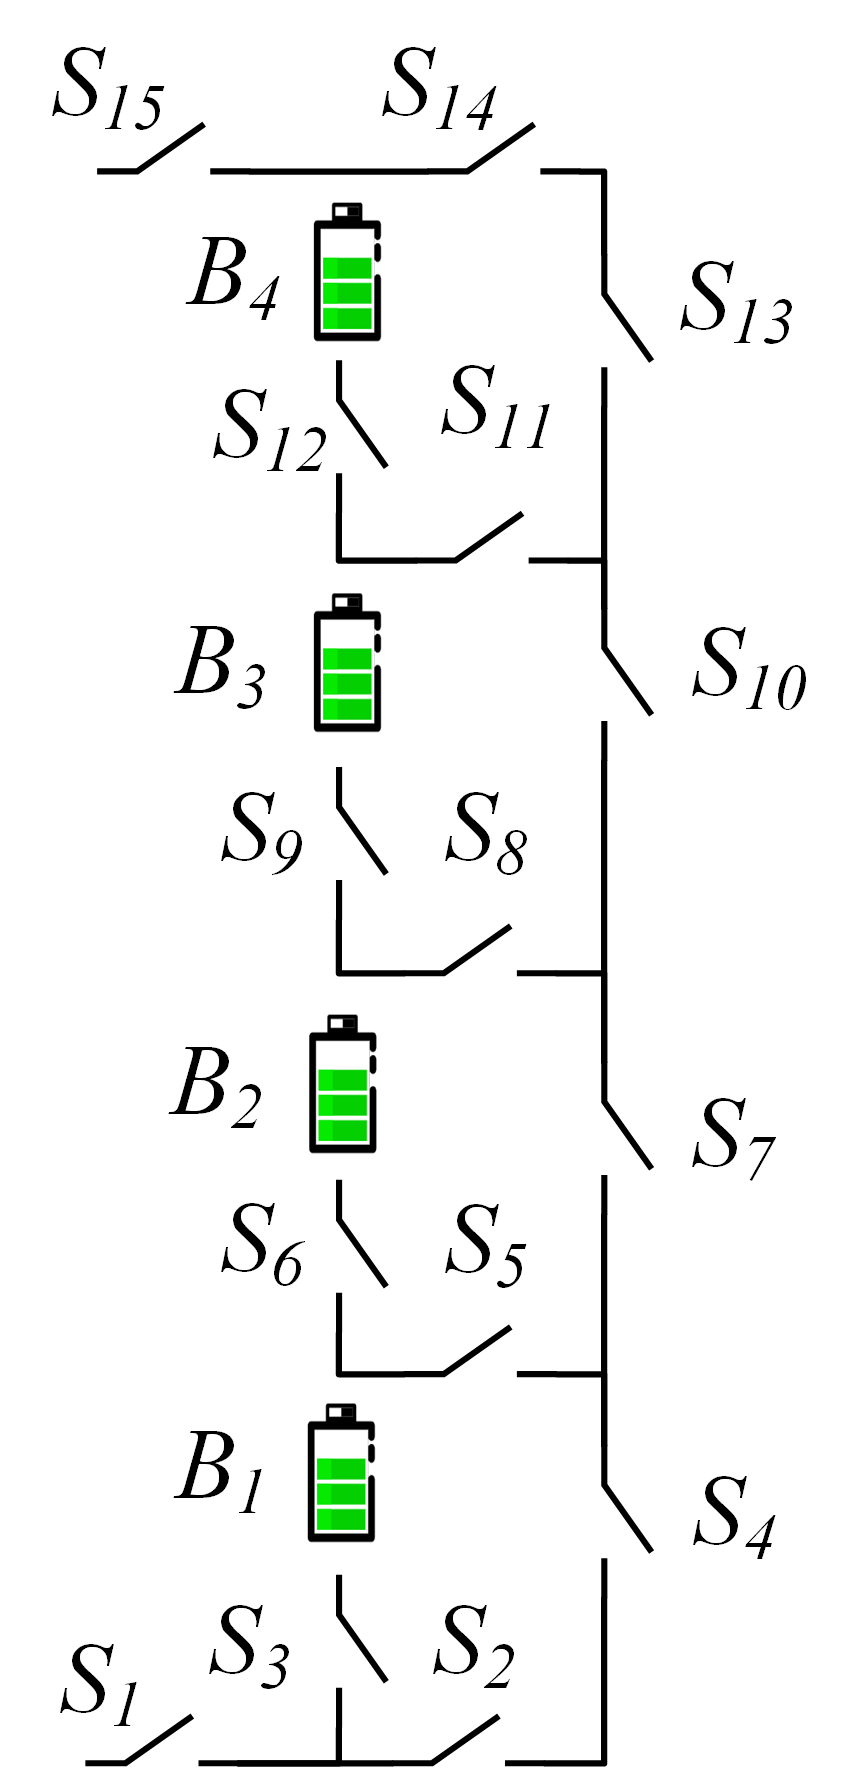
\includegraphics[width=\textwidth]{stru-L-origin.png}
        \caption{}
        \label{fig:study-stru-Lawson}
    \end{subfigure}
    \hspace{0.02\textwidth}
    \begin{subfigure}[b]{0.4\textwidth}
        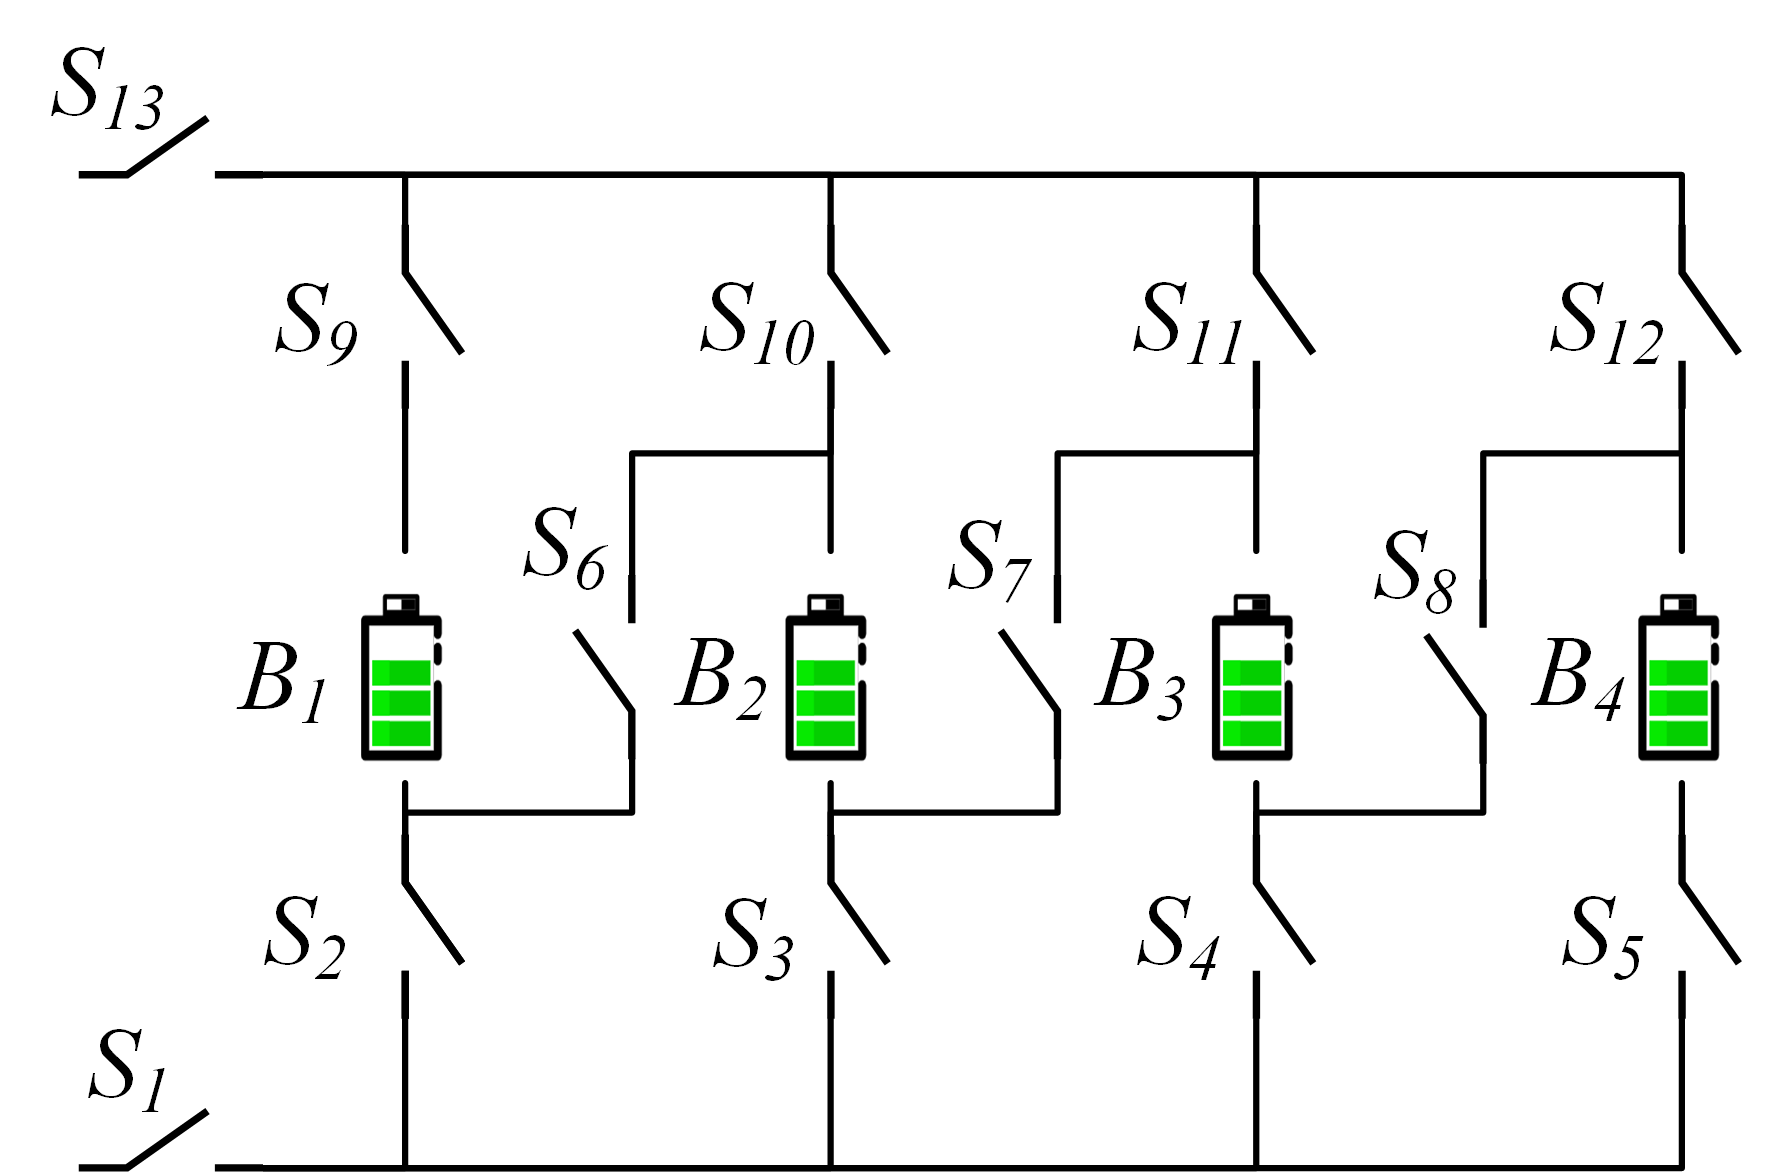
\includegraphics[width=\textwidth]{stru-V-origin.png}
        \caption{}
        \label{fig:study-stru-Visairo}
    \end{subfigure}
    \hspace{0.02\textwidth}
    \begin{subfigure}[b]{0.31\textwidth}
        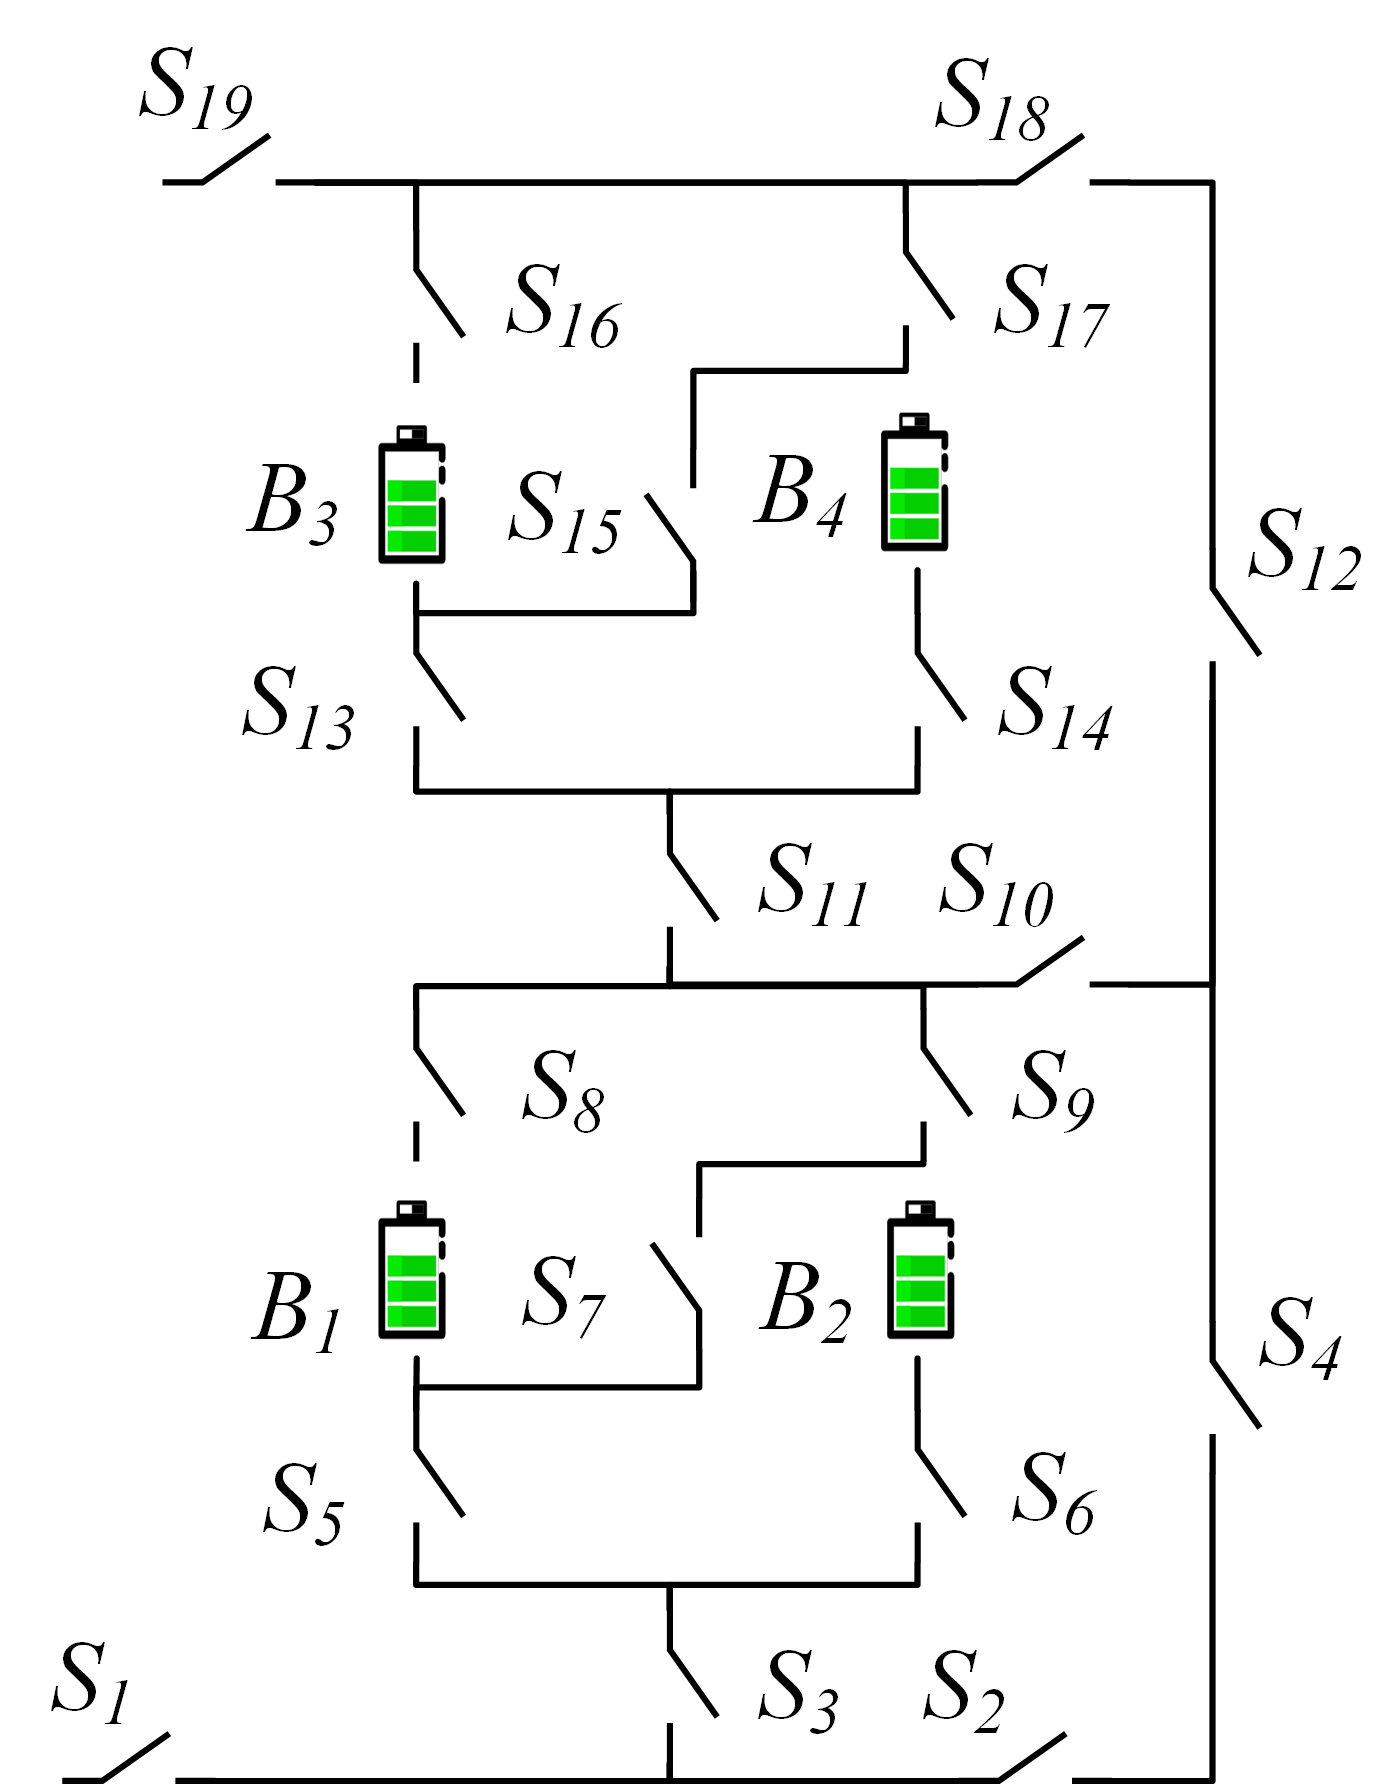
\includegraphics[width=\textwidth]{stru-my-origin.png}
        \caption{}
        \label{fig:study-stru-my}
    \end{subfigure}
    \caption{The four-battery RBS structures proposed by (a) Lawson \cite{lawsonSoftwareConfigurableBattery2012}, (b) Visairo \cite{visairoReconfigurableBatteryPack2008}, and (c) this paper.}
\end{figure}

Currently, two types of RBS structures have been proposed by Visairo et al. \cite{visairoReconfigurableBatteryPack2008} and Lawson et al. \cite{lawsonSoftwareConfigurableBattery2012}, both of which have seen real use. 
The primary goal of Visairo's structure (Fig. \ref{fig:study-stru-Visairo}) is to dynamically adjust the RBS output power. However, the isolation of unhealthy batteries is not sufficiently addressed in their work. 
Lawson et al. designed the RBS structure shown in Fig. \ref{fig:study-stru-Lawson} to isolate batteries. 
Although this structure easily isolates batteries, it cannot dynamically adjust the output current of the RBS. 
Based on the structures of Visairo and Lawson, this paper proposes the structure shown in Fig. \ref{fig:study-stru-my}.
By integrating the Visairo RBS structure into the Lawson RBS structure, the proposed structure not only has the flexibility to switch the batteries between series, parallel, and mixed series-parallel modes but also allows the isolation of highly degraded batteries from the RBS.


In the case study, these RBS systems are investigated and compared: (a) three different structures (Figs. \ref{fig:study-stru-Lawson}--\ref{fig:study-stru-my}) with the same four batteries; (b) the same structure in Figs. \ref{fig:study-stru-my} with two/four/six batteries; and (c) the four-battery structure in Figs. \ref{fig:study-stru-my} with random isolated batteries. 
The greedy algorithm proposed in this work is also compared with the brute-force algorithm, SA, and GA to validate its effectiveness and efficiency.
In order to adapt the two heuristic algorithms to the system's structure and scale, the number of the state neighbours of SA and the population size of GA are both set to $N_b \cdot N_s$, which increase with the number of batteries and switches in the system. 
The other algorithms' parameters are shown in Tab. \ref{tab:algorithm-parameter}.

\begin{table}[htbp]
  \centering
  \caption{Algorithms parameters of SA and GA.}
    \begin{tabular}{lr}
    \toprule
    Algorithm/paramter & \multicolumn{1}{l}{Value} \\
    \midrule
    SA/initial temperature & 100 \\
    SA/final temperature & 1 \\
    SA/cooling rate & 0.95 \\
    GA/total generations & 100 \\
    GA/crossover probability & 0.8 \\
    GA/mutation probability & 0.02 \\
    \bottomrule
    \end{tabular}
  \label{tab:algorithm-parameter}
\end{table}

\subsection{Result}

\subsubsection{the shortest path}

Using Eq. (\ref{eq:weight}) and the Dijkstra algorithm, the SPs of the four batteries in the RBS structures of Figs. \ref{fig:study-stru-Lawson}, \ref{fig:study-stru-Visairo}, and \ref{fig:study-stru-my} are calculated and highlighted with difference colors in Figs. \ref{fig:e4-sp}, \ref{fig:f4-sp}, and \ref{fig:e2f2-sp}, respectively.

\begin{figure}[htbp]
    \centering
    \begin{subfigure}[b]{0.2\textwidth}
        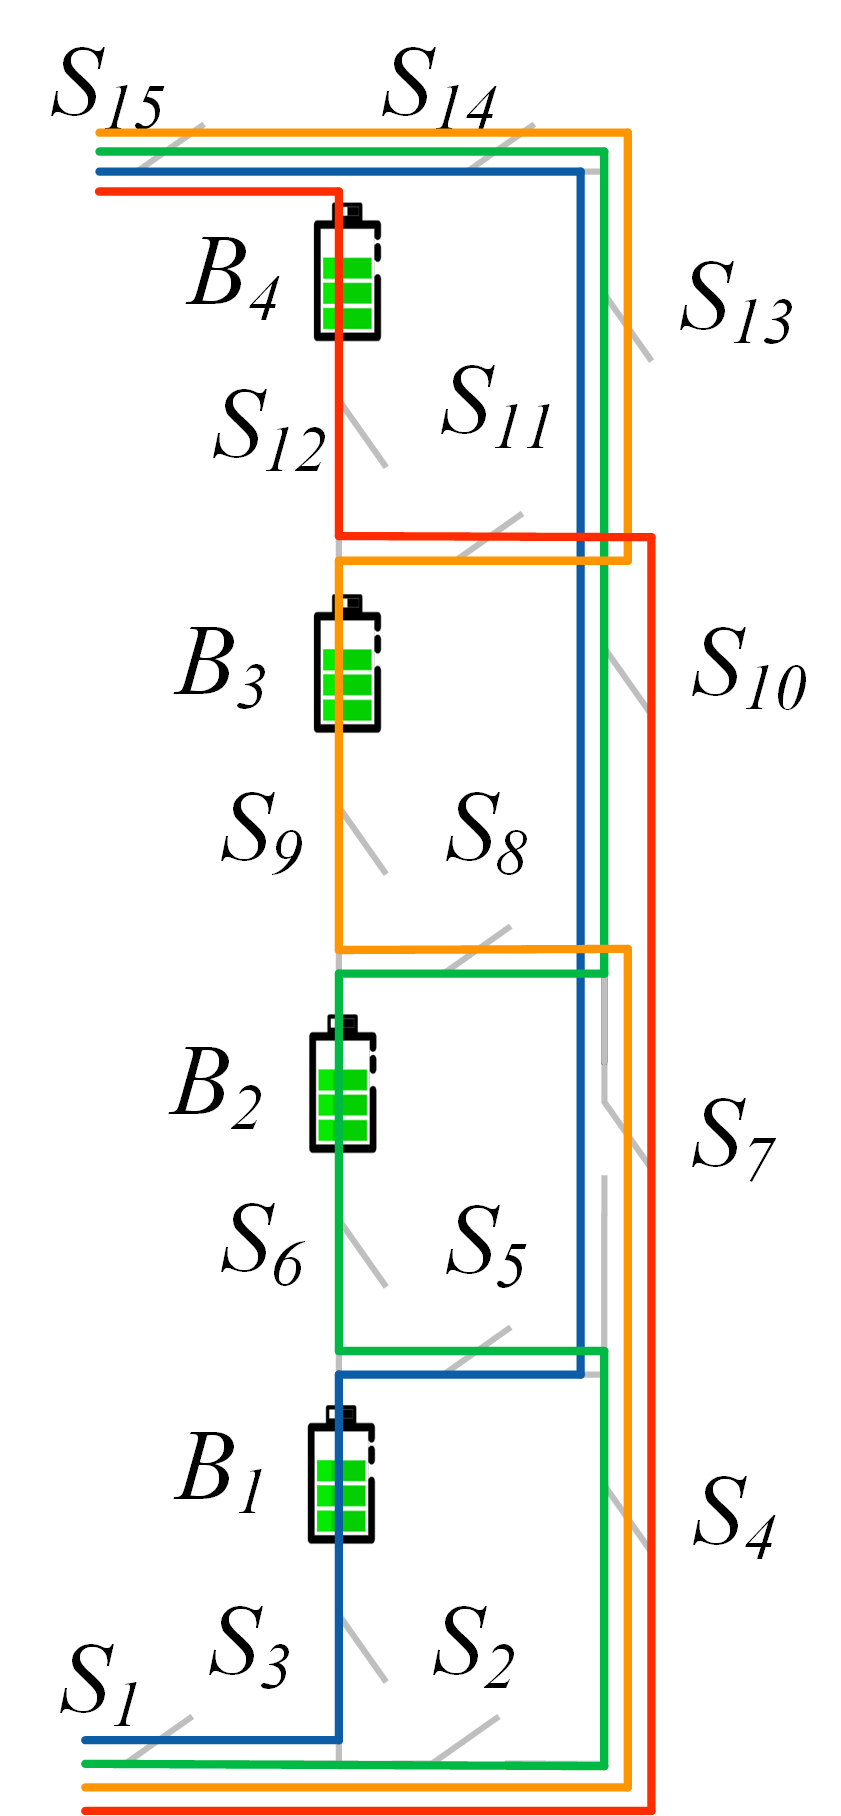
\includegraphics[width=\textwidth]{e4-sp.png}
        \caption{}
        \label{fig:e4-sp}
    \end{subfigure}
    \hspace{0.02\textwidth}
    \begin{subfigure}[b]{0.4\textwidth}
        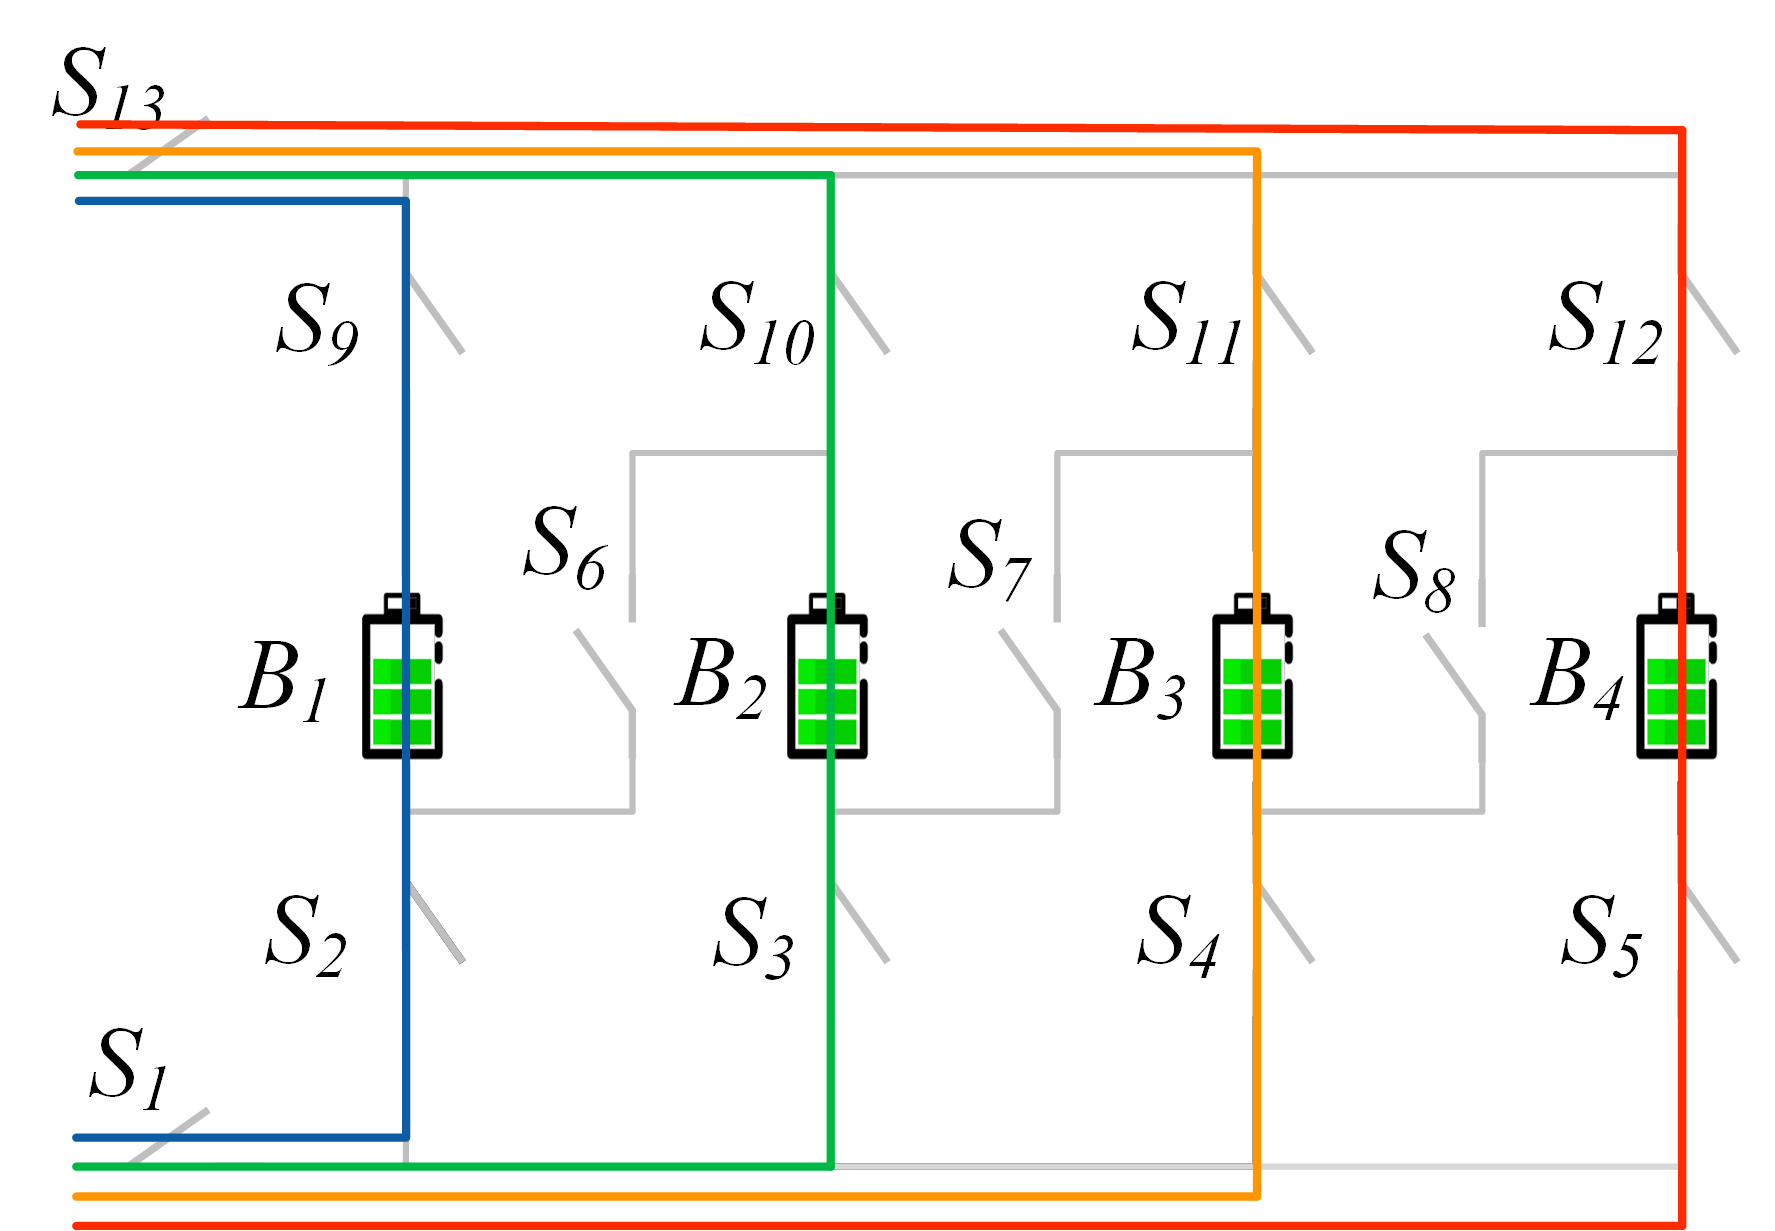
\includegraphics[width=\textwidth]{f4-sp.png}
        \caption{}
        \label{fig:f4-sp}
    \end{subfigure}
    \hspace{0.02\textwidth}
    \begin{subfigure}[b]{0.31\textwidth}
        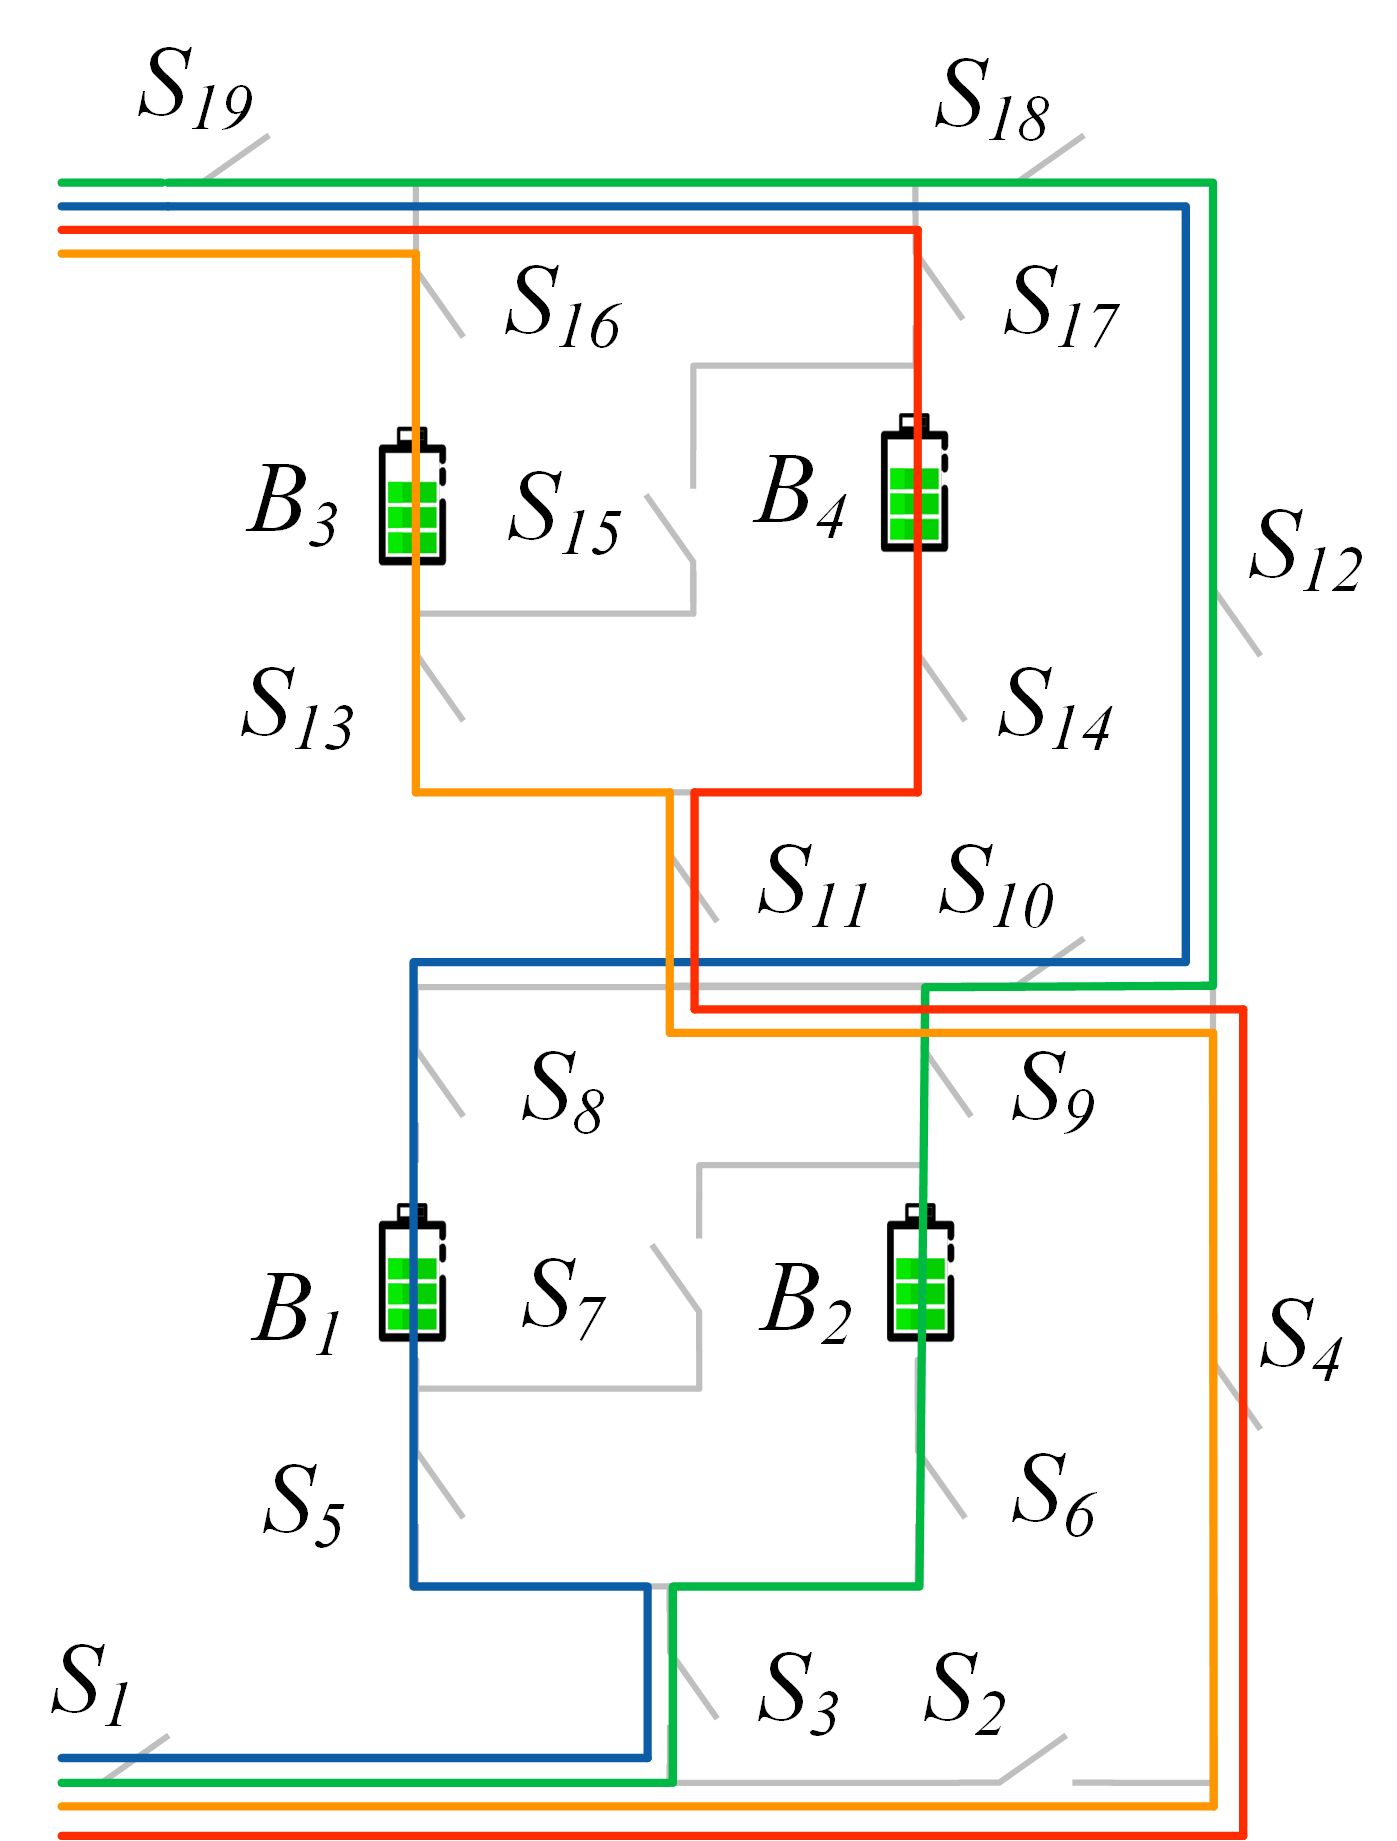
\includegraphics[width=\textwidth]{e2f2-sp.png}
        \caption{}
        \label{fig:e2f2-sp}
    \end{subfigure}
    \caption{The SPs of the four batteries in the RBS structures of (a) Fig. \ref{fig:study-stru-Lawson}, (b) Fig. \ref{fig:study-stru-Visairo}, and (c) Fig. \ref{fig:study-stru-my}.}
\end{figure}

\subsubsection{three structures with four batteries}

After obtaining the SPs, the MACs of the three RBS structures with four batteries are calculated using the proposed greedy algorithm, and the results are shown in Tabs. \ref{tab:study-results-Lawson}, \ref{tab:study-results-Visairo}, and \ref{tab:study-results-my}, each of which contains the states of the switches, the output current $I_o$, the battery current $\bm{I}_b$, and the ratio $\eta$ when the system output reaches the MAC.
The correspond switch-control schemes are shown as blue-highlighted electric current in Figs. \ref{fig:e4-mac}, \ref{fig:f4-mac}, and \ref{fig:e2f2-mac}, respectively.
To verify and compare the proposed greedy algorithm, we also used the brute-force algorithm, which iterates through all possible switch states, and the heuristic algorithms (SA and GA) to calculate the MAC of the same RBSs. 
The final results of the brute-force algorithm are the same as the ones of the greedy algorithm, which are shown in Tabs. \ref{tab:study-results-Lawson}, \ref{tab:study-results-Visairo}, and \ref{tab:study-results-my}.
But, the brute-force algorithm counts all possible switch states, which equates to $2^{15}$, $2^{13}$, and $2^{19}$ structures, respectively.
The two heuristic algorithms' temporal evaluation of the objective values during the iteration process are shown in Figs. \ref{fig:e4-alg}, \ref{fig:f4-alg}, and \ref{fig:e2f2-alg}, respectively, compared with the proposed greedy algorithm.

\begin{table}[htbp]
  \centering
    \caption{MAC Calculating result of the four-battery RBS structure in Fig. \ref{fig:study-stru-Lawson}.}
    \begin{tabular}{cc}
    \toprule
        Structure & Figure \ref{fig:study-stru-Lawson} with 4 batteries and 15 switches  \\
    \midrule
    Switch ON & $S_1$,$S_3$,$S_5$,$S_7$,$S_{10}$,$S_{13}$,$S_{14}$,$S_{15}$ \\
    $I_o$ & $u_b/(R_o+r_b)$ \\
    $\bm{I}_b$ & $[u_b/(R_o+r_b),0,0,0]$ \\
    $\max \eta$     & 1 \\
    \bottomrule
    \end{tabular}
  \label{tab:study-results-Lawson}
\end{table}

\begin{table}[htbp]
  \centering
    \caption{MAC Calculating result of the four-battery RBS structure in Fig. \ref{fig:study-stru-Visairo}.}
    \begin{tabular}{cc}
    \toprule
        Structure & Figure \ref{fig:study-stru-Visairo} with 4 batteries and 13 switches  \\
    \midrule
    Switch ON & $S_1$,$S_2$,$S_3$,$S_4$,$S_5$,$S_9$,$S_{10}$,$S_{11}$,$S_{12}$,$S_{13}$ \\
    $I_o$ & $4u_b/(4R_o+r_b)$ \\
    $\bm{I}_b$ & $[u_b/(4R_o+r_b),u_b/(4R_o+r_b),u_b/(4R_o+r_b),u_b/(4R_o+r_b)]$ \\
    $\max \eta$     & 4 \\
    \bottomrule
    \end{tabular}
  \label{tab:study-results-Visairo}
\end{table}

\begin{table}[htbp]
  \centering
    \caption{Calculated MAC for four-battery RBS structure in Fig. \ref{fig:study-stru-my}.}
    \begin{tabular}{cc}
    \toprule
        Structure & Figure \ref{fig:study-stru-my} with four batteries and 19 switches  \\
    \midrule
    Switch on & $S_1$,$S_3$,$S_5$,$S_6$,$S_8$,$S_9$,$S_{10}$,$S_{12}$,$S_{18}$,$S_{19}$ \\
    $I_o$ & $2u_b/(2R_o+r_b)$ \\
    $\bm{I}_b$ & $[u_b/(2R_o+r_b),u_b/(2R_o+r_b),0,0]$ \\
    $\max \eta$     & 2 \\
    \bottomrule
    \end{tabular}
  \label{tab:study-results-my}
\end{table}
  
\begin{figure}[htbp]
    \centering
    \begin{subfigure}[b]{0.2\textwidth}
        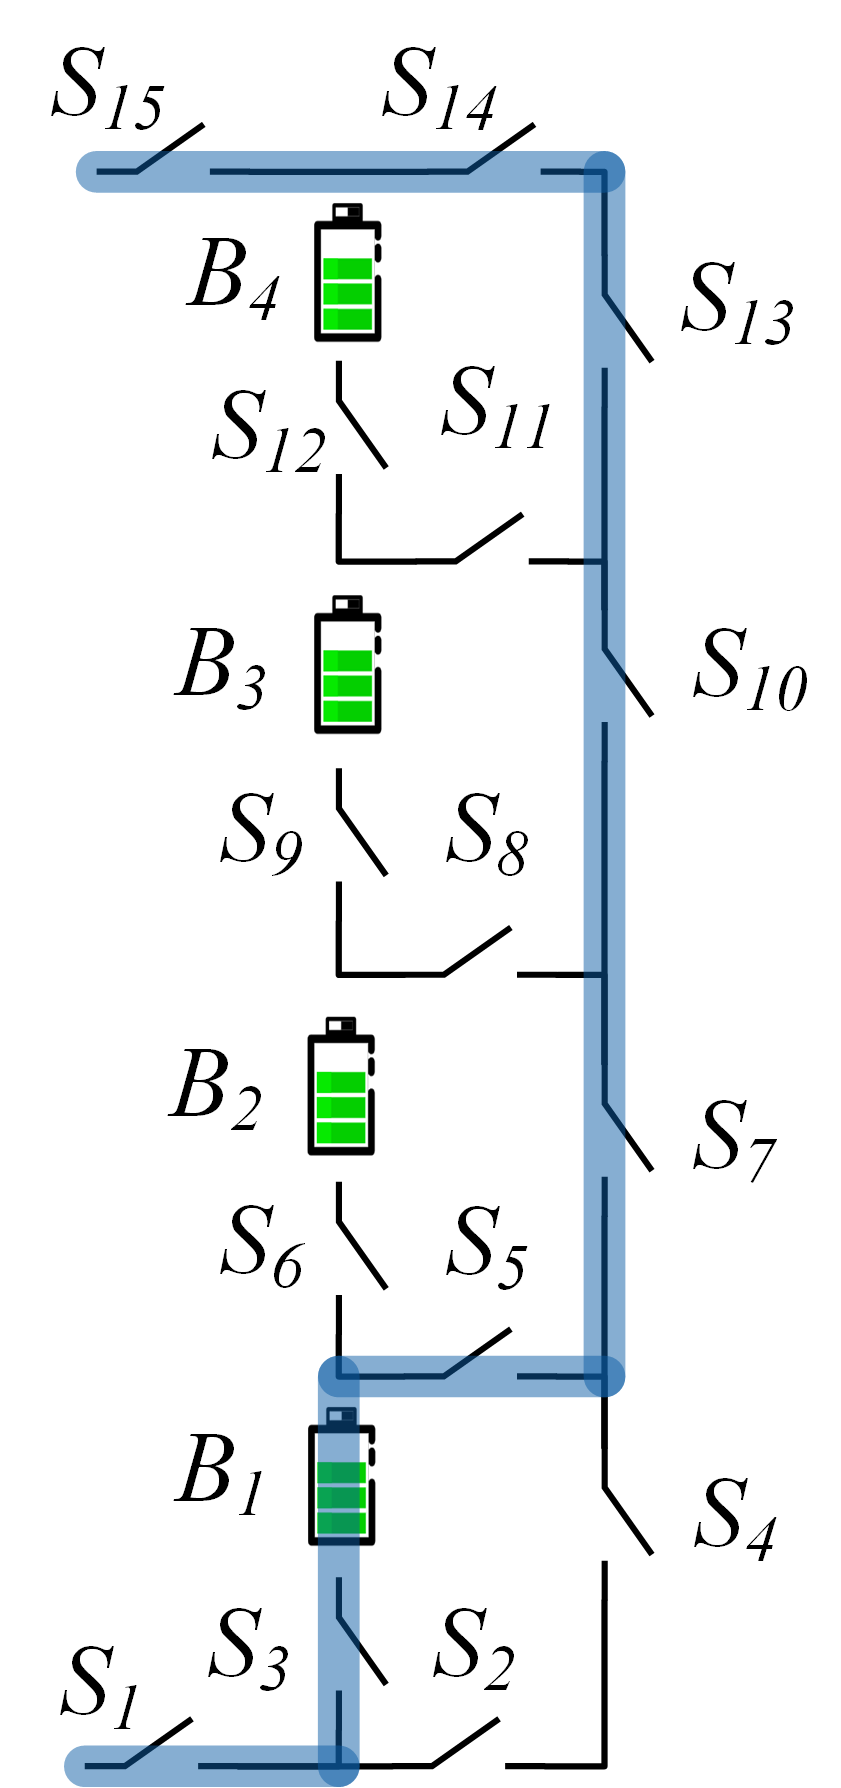
\includegraphics[width=\textwidth]{e4-mac.png}
        \caption{}
        \label{fig:e4-mac}
    \end{subfigure}
    \hspace{0.02\textwidth}
    \begin{subfigure}[b]{0.4\textwidth}
        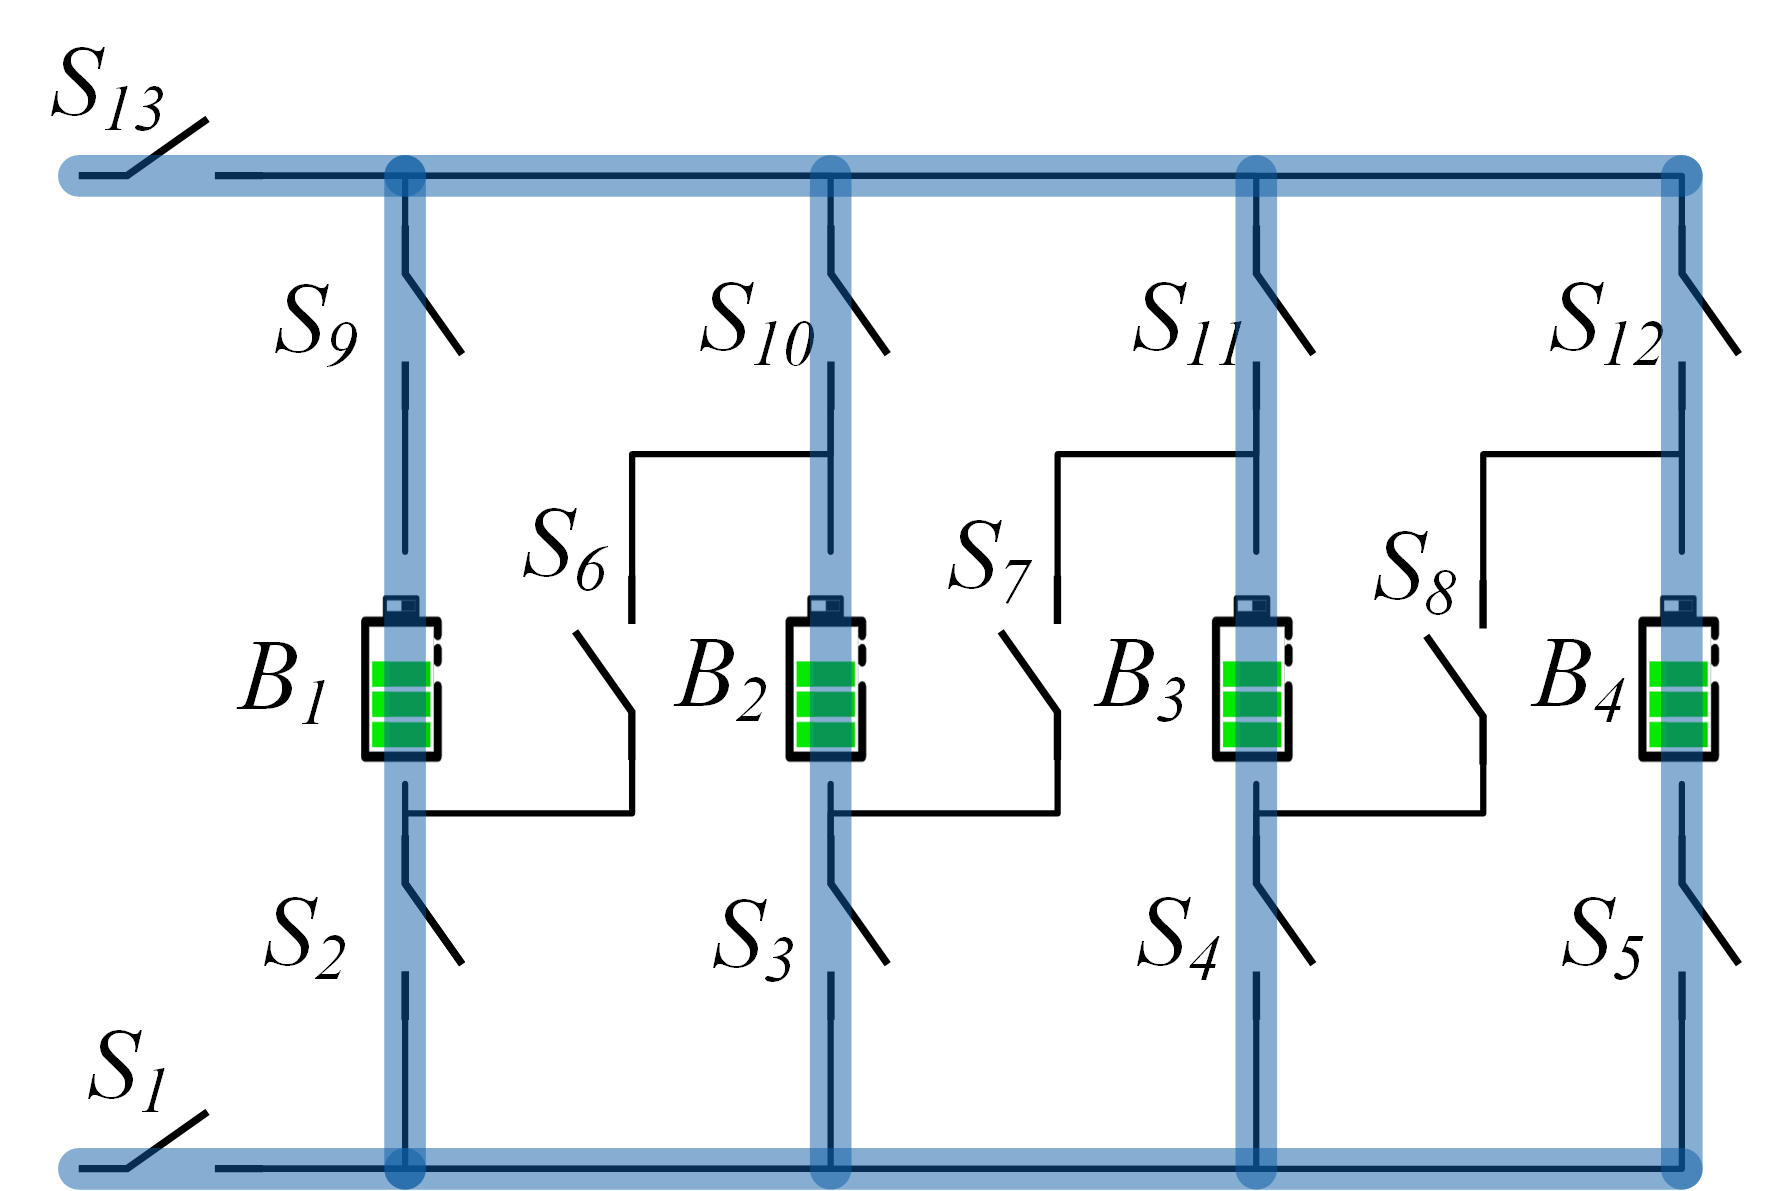
\includegraphics[width=\textwidth]{f4-mac.png}
        \caption{}
        \label{fig:f4-mac}
    \end{subfigure}
    \hspace{0.02\textwidth}
    \begin{subfigure}[b]{0.31\textwidth}
        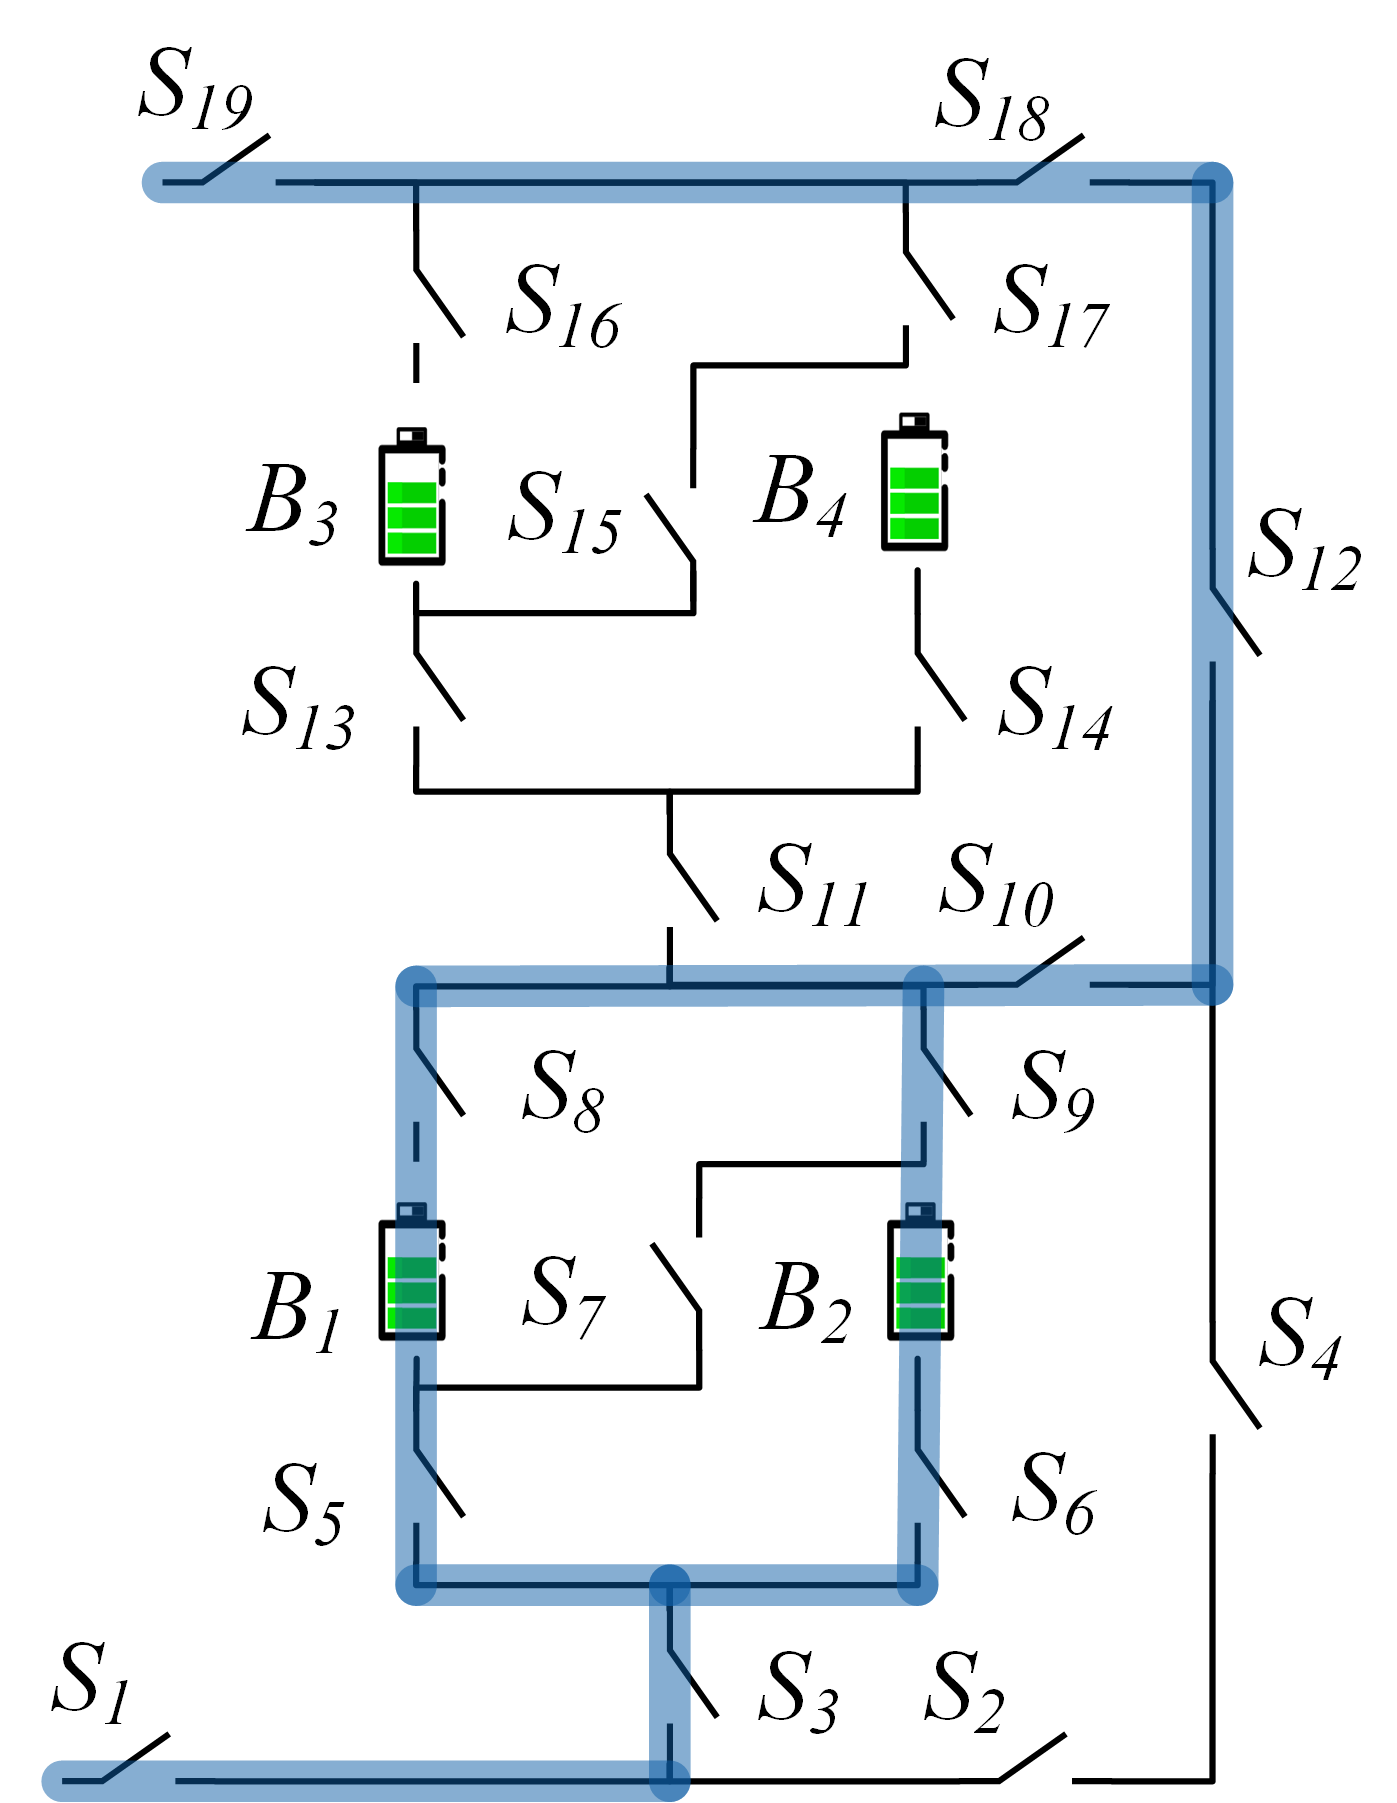
\includegraphics[width=\textwidth]{e2f2-mac.png}
        \caption{}
        \label{fig:e2f2-mac}
    \end{subfigure}
    \caption{The RBSs' switch-control schemes with the output reaching the MAC.}
\end{figure}

\begin{figure}[htbp]
    \centering
    \begin{subfigure}[b]{0.32\textwidth}
        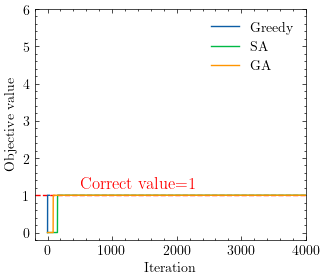
\includegraphics[width=\textwidth]{e4-alg.png}
        \caption{}
        \label{fig:e4-alg}
    \end{subfigure}
    % \hspace{0.02\textwidth}
    \begin{subfigure}[b]{0.32\textwidth}
        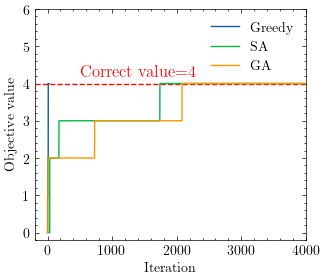
\includegraphics[width=\textwidth]{f4-alg}
        \caption{}
        \label{fig:f4-alg}
    \end{subfigure}
    % \hspace{0.02\textwidth}
    \begin{subfigure}[b]{0.32\textwidth}
        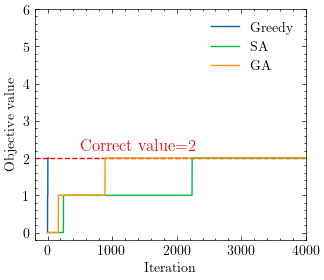
\includegraphics[width=\textwidth]{e2f2-alg}
        \caption{}
        \label{fig:e2f2-alg}
    \end{subfigure}
    \caption{The temporal evolution of the objective values during the iteration process of calculating the RBS structures in (a) Fig. \ref{fig:study-stru-Lawson}, (b) Fig. \ref{fig:study-stru-Visairo}, and (c) Fig. \ref{fig:study-stru-my}}
\end{figure}

\subsubsection{structures with different numbers of batteries}

We next consider the RBS structure in Fig. \ref{fig:study-stru-my} with two, four, and six batteries.
The result of four-battery structure has been shown in Tab. \ref{tab:study-results-my}, Figs. \ref{fig:e2f2-mac}, and \ref{fig:e2f2-alg}. 
The structures and final switch-control schemes of the remaining two-battery and six-battery systems are illustrated in Figs. \ref{fig:e2f1-mac} and \ref{fig:e2f3-mac}, respectively. 
And the temporal evolution of the objective values throughout the iteration process are shown in Figs. \ref{fig:e2f1-alg} and \ref{fig:e2f3-alg}, respectively.

\begin{figure}[htbp]
    \centering
    \begin{subfigure}[b]{0.27\textwidth}
        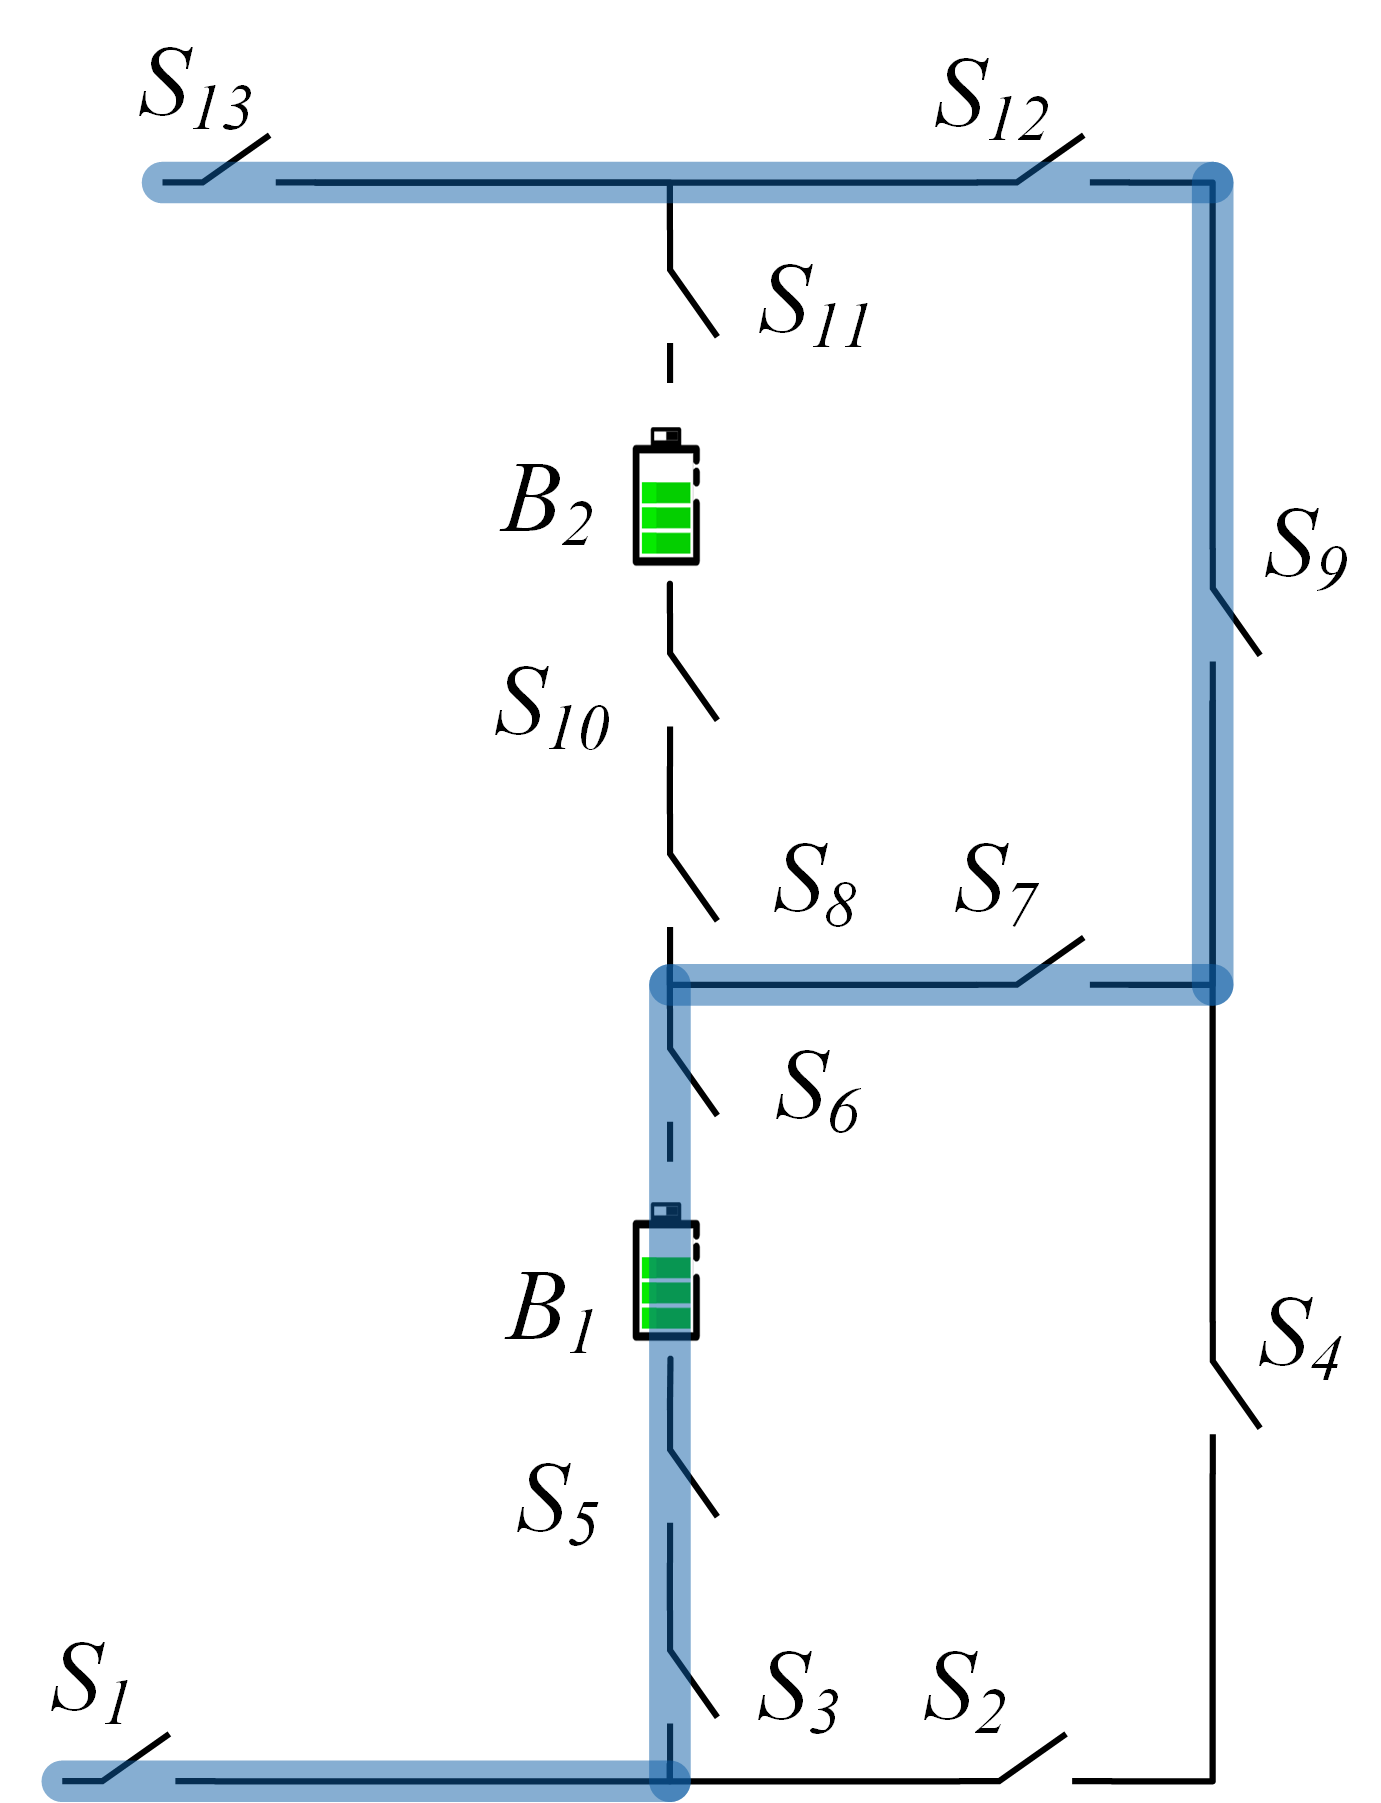
\includegraphics[width=\textwidth]{e2f1-mac.png}
        \caption{}
        \label{fig:e2f1-mac}
    \end{subfigure}
    \hspace{0.02\textwidth}
    \begin{subfigure}[b]{0.31\textwidth}
        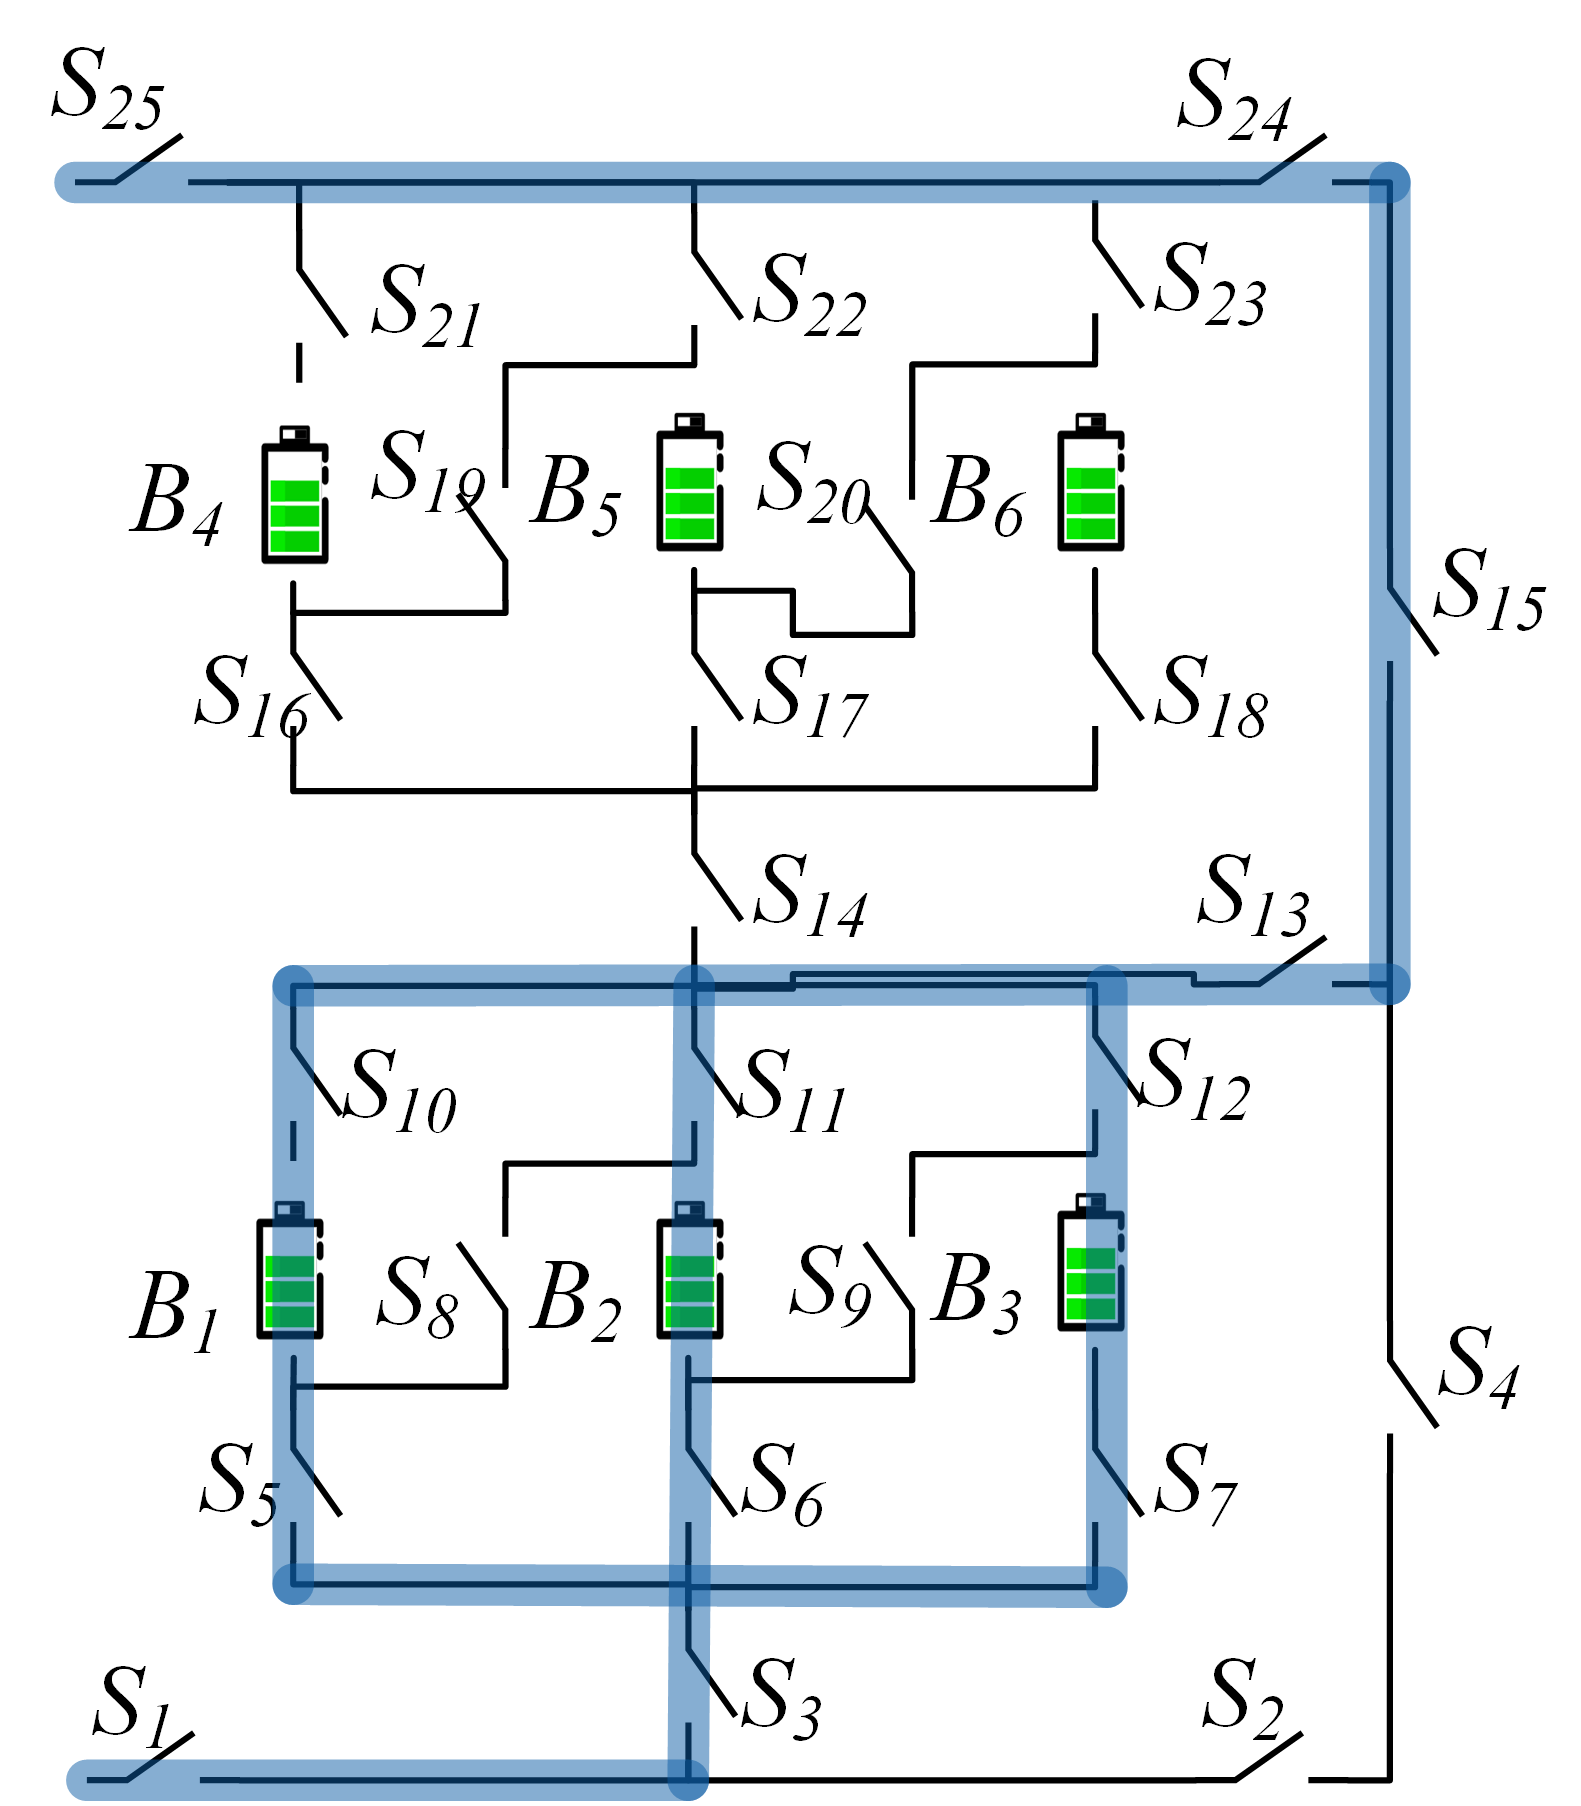
\includegraphics[width=\textwidth]{e2f3-mac.png}
        \caption{}
        \label{fig:e2f3-mac}
    \end{subfigure}
    \caption{The (a) two-battery and (b) six-battery RBSs' switch-control schemes with the output reaching the MAC.}
\end{figure}

\begin{figure}[htbp]
    \centering
    \begin{subfigure}[b]{0.34\textwidth}
        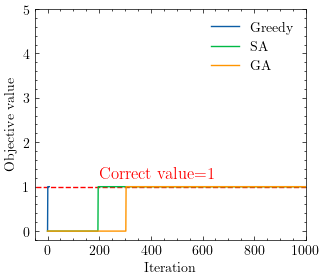
\includegraphics[width=\textwidth]{e2f1-alg.png}
        \caption{}
        \label{fig:e2f1-alg}
    \end{subfigure}
    \hspace{0.02\textwidth}
    \begin{subfigure}[b]{0.33\textwidth}
        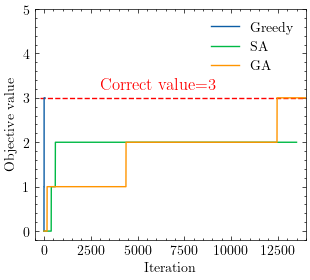
\includegraphics[width=\textwidth]{e2f3-alg.png}
        \caption{}
        \label{fig:e2f3-alg}
    \end{subfigure}
    \caption{The temporal variation of the objective values during the iteration process of calculating the RBS structures in (a) Fig. \ref{fig:e2f1-mac} and (b) Fig. \ref{fig:e2f3-mac}.}
\end{figure}

\subsubsection{random isolated batteries}

To assess the effectiveness of the proposed algorithm in the scenario of unhealthy batteries, the RBS with random isolated batteries is also taken into account and computed. 
In the case of the four-battery RBS structure depicted in Fig. \ref{fig:study-stru-my}, there are four possible scenarios of isolated batteries: (a) only one unhealthy battery, (b) two unhealthy batteries that are separated in the two substructure, (c) two batteries located in the same substructure, and (d) three batteries. 
The resulting MAC ($\eta$) values for these four scenarios are 2, 2, 1, and 1, respectively.
Furthermore, the corresponding switch-control schemes for these four scenarios are illustrated in Figs \ref{fig:my-isolated-1}--\ref{fig:my-isolated-3}.

\begin{figure}[htbp]
    \centering
    \begin{subfigure}[b]{0.31\textwidth}
        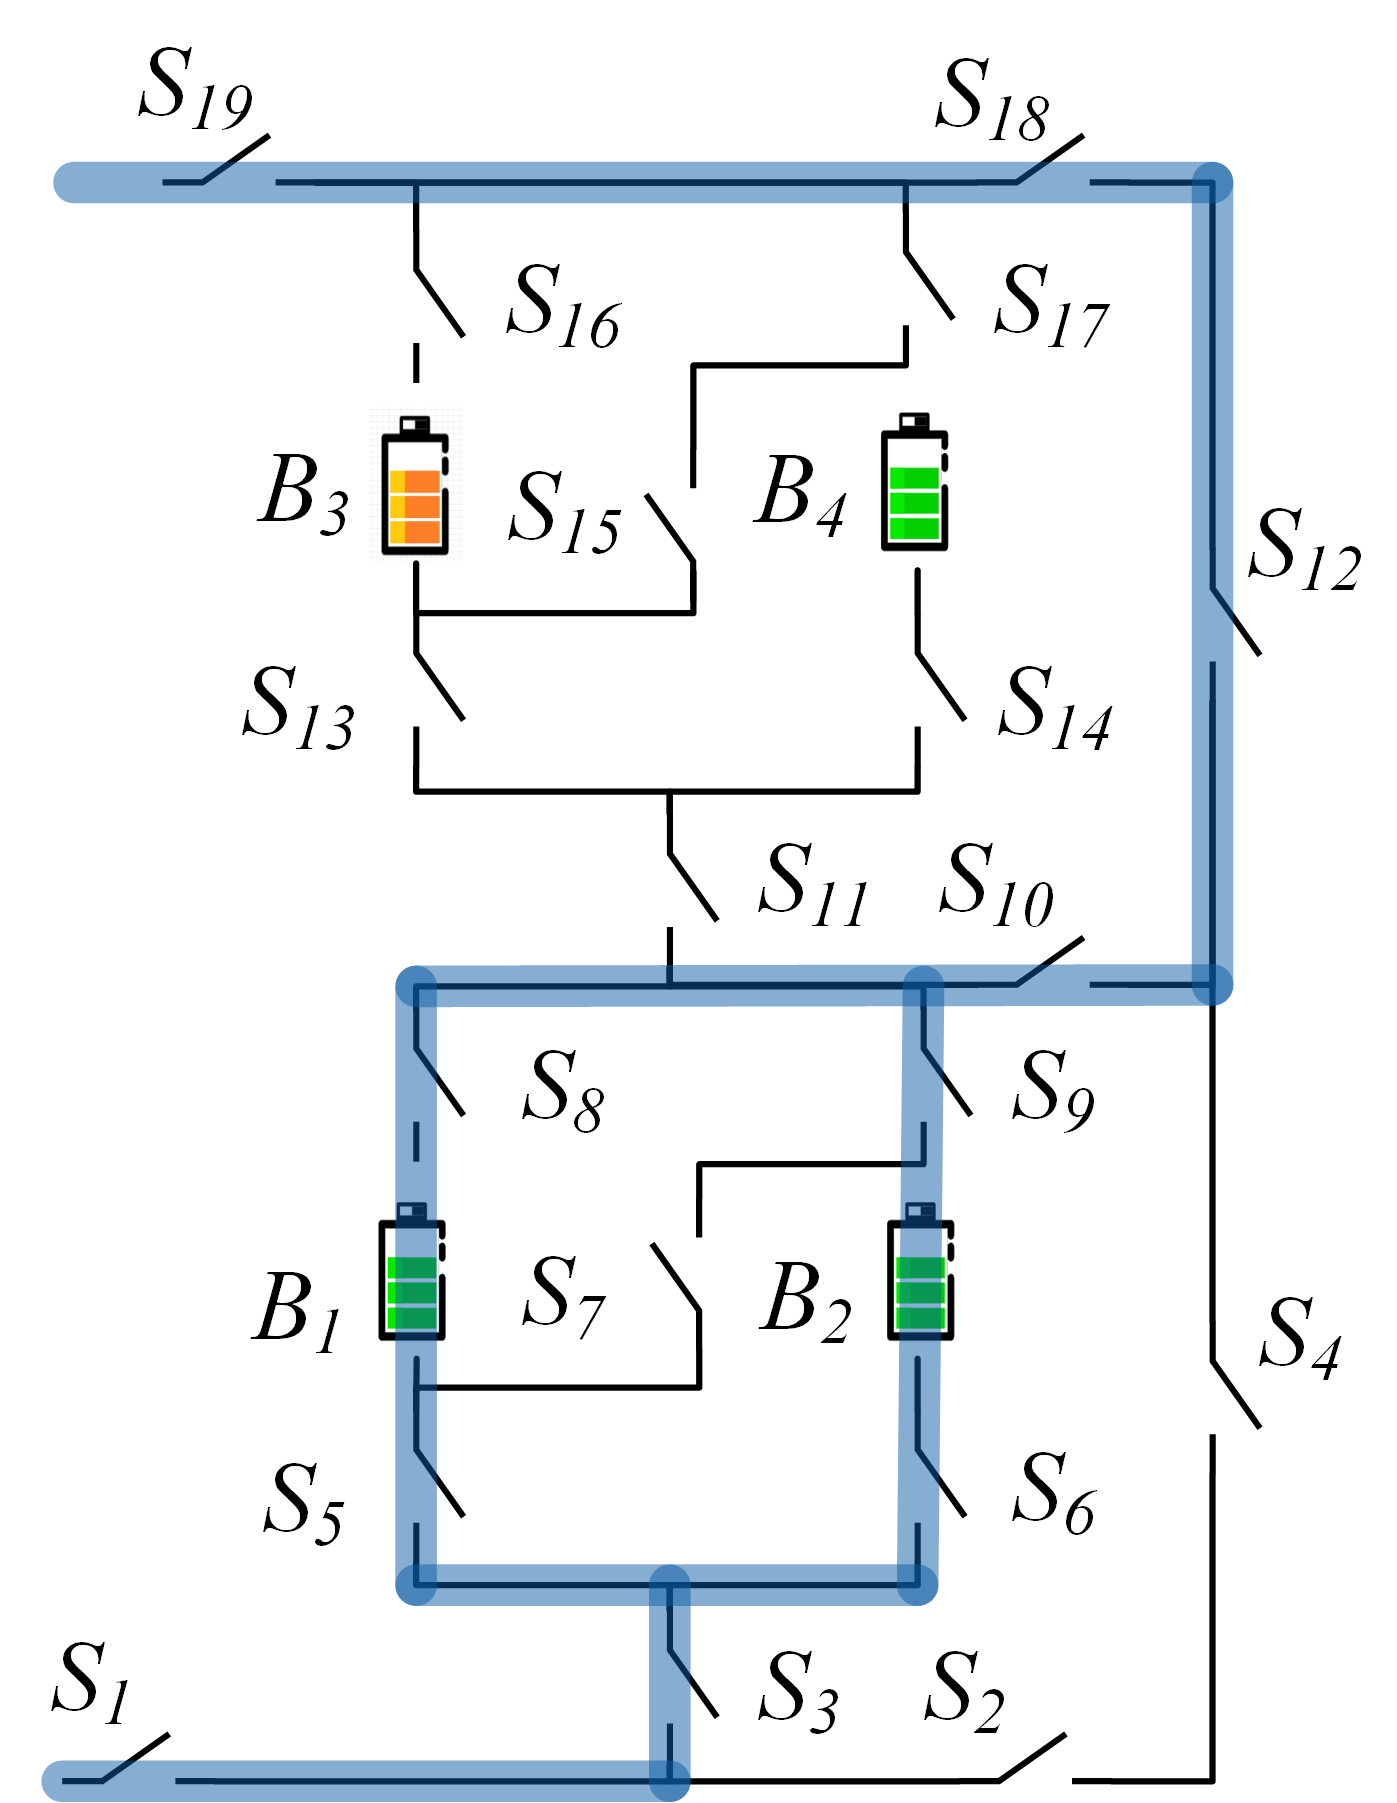
\includegraphics[width=\textwidth]{e2f2-isolate-1.png}
        \caption{}
        \label{fig:my-isolated-1}
    \end{subfigure}
    \hspace{0.02\textwidth}
    \begin{subfigure}[b]{0.31\textwidth}
        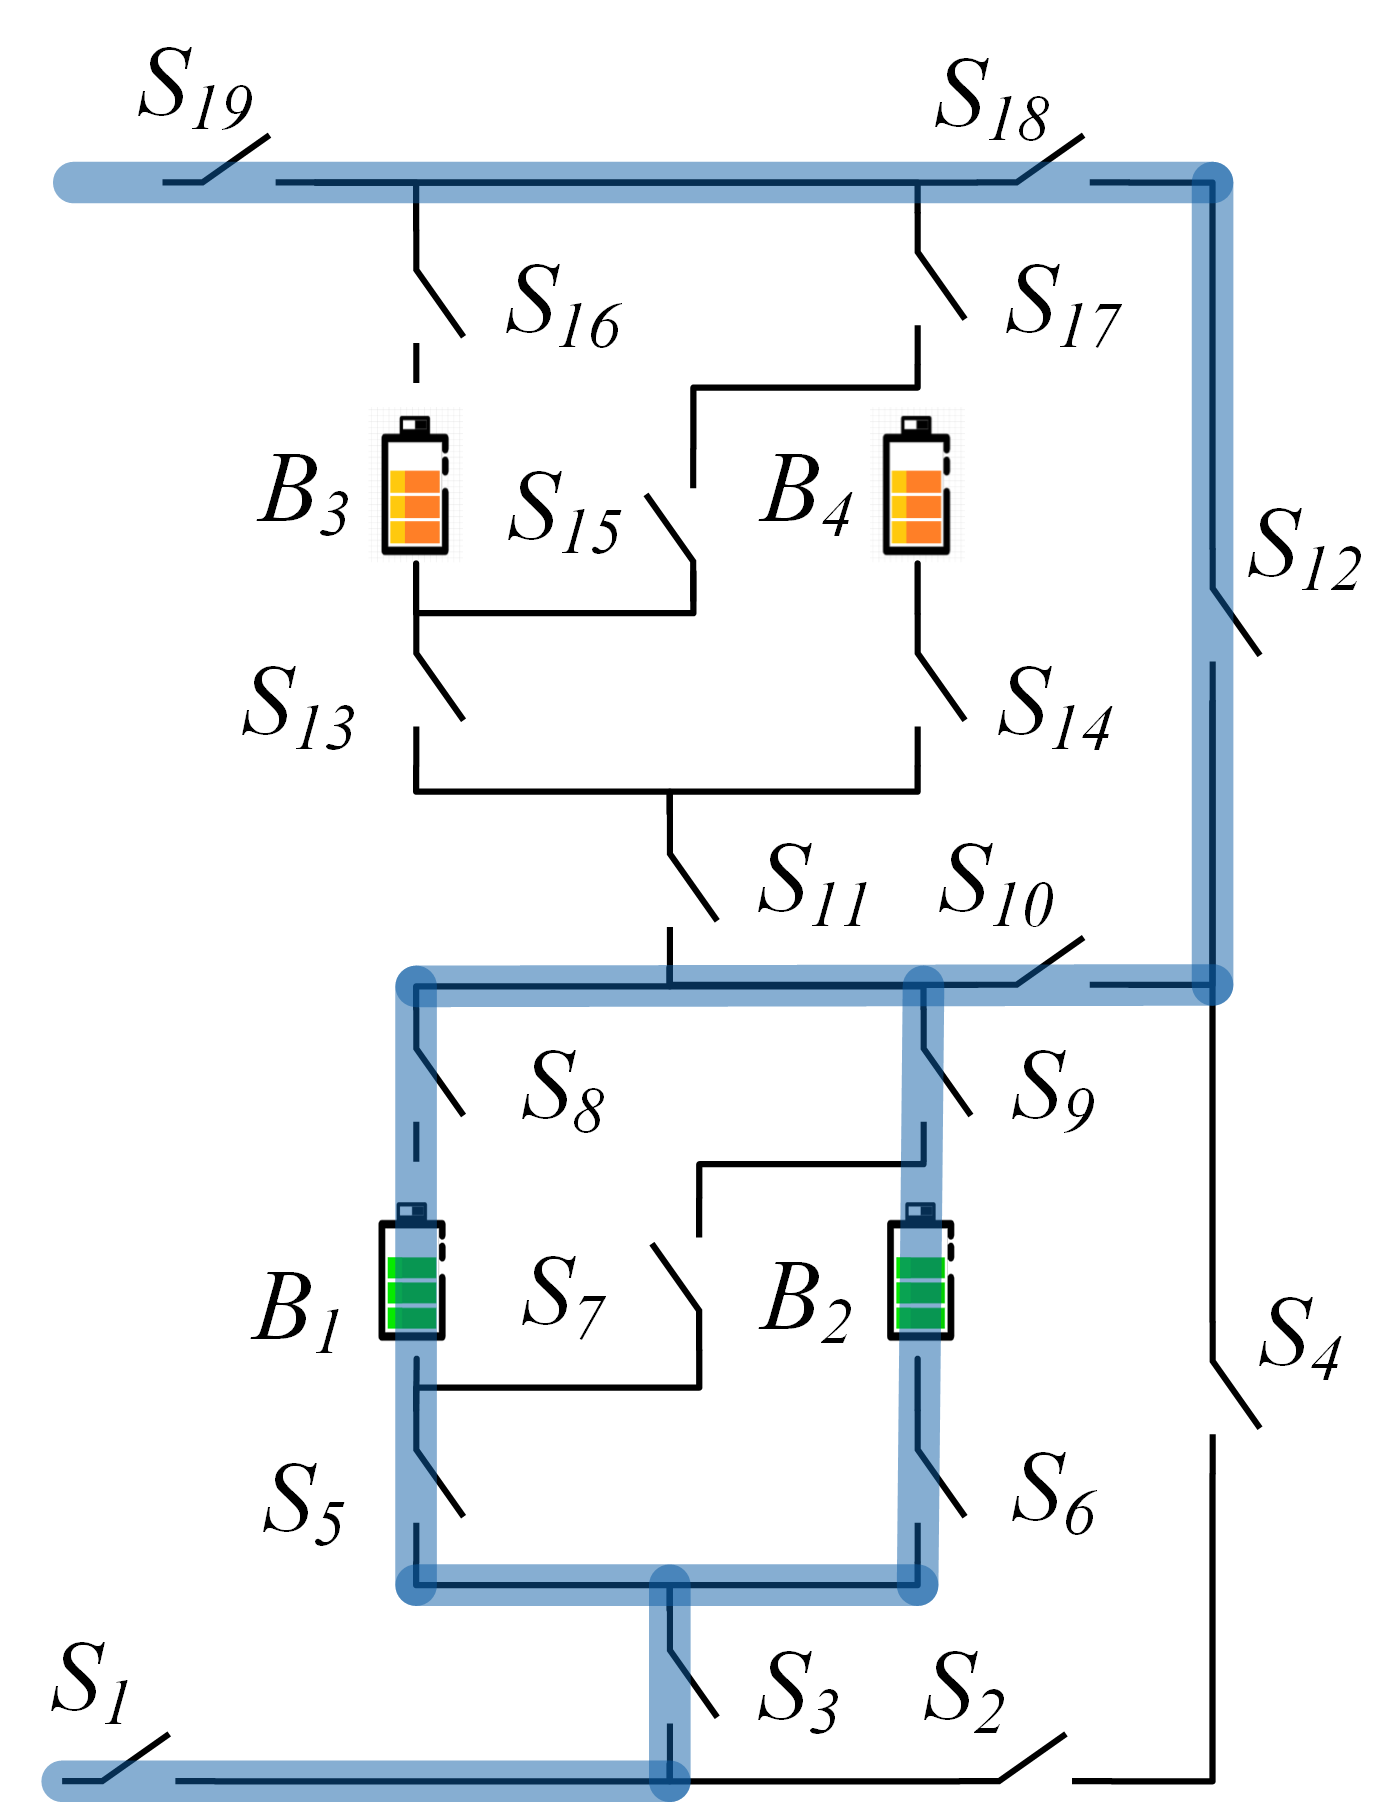
\includegraphics[width=\textwidth]{e2f2-isolate-2b.png}
        \caption{}
        \label{fig:my-isolated-2b}
    \end{subfigure}
    \\
    \begin{subfigure}[b]{0.31\textwidth}
        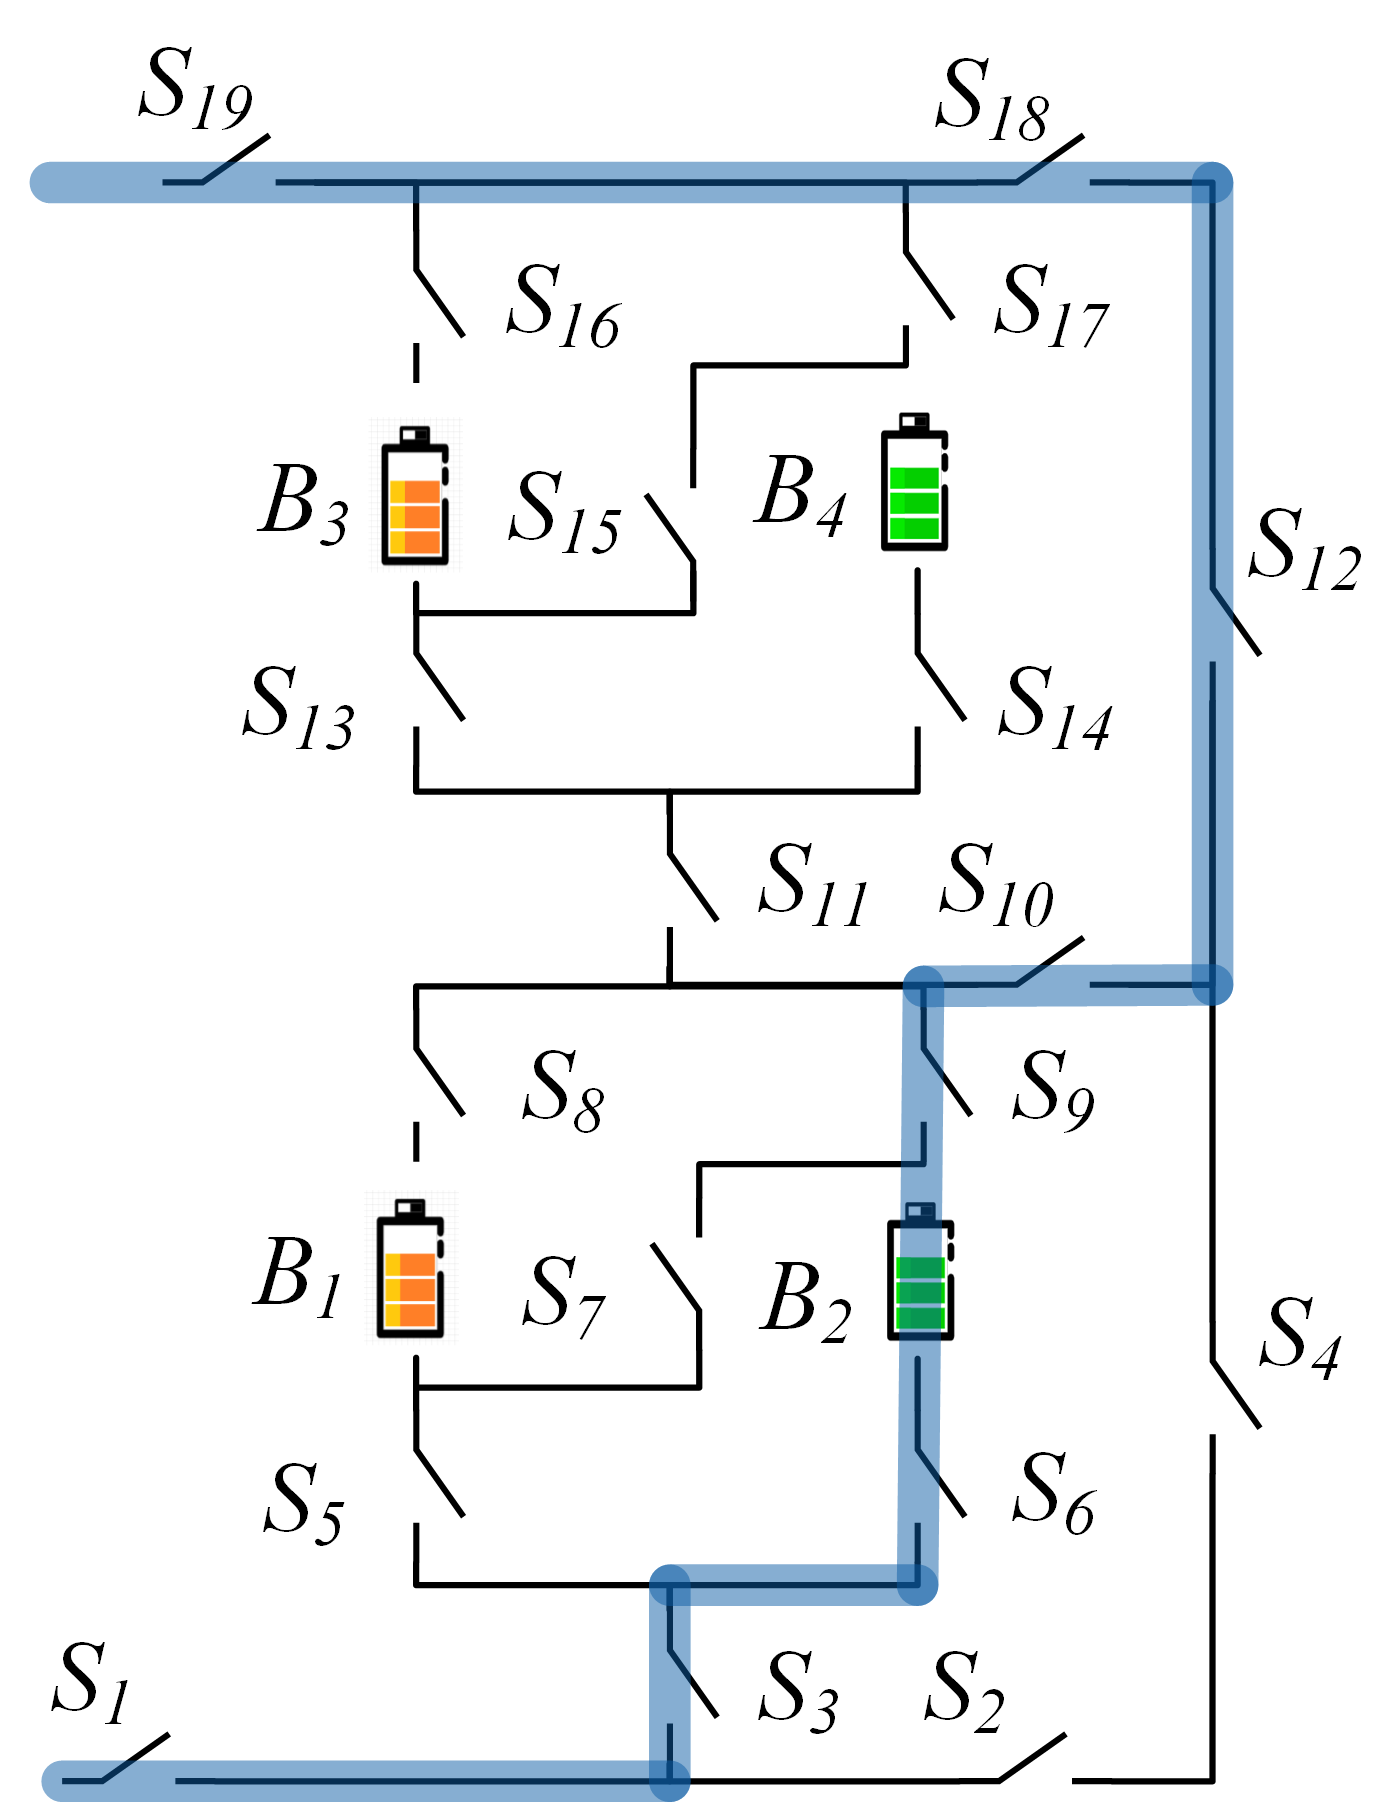
\includegraphics[width=\textwidth]{e2f2-isolate-2w.png}
        \caption{}
        \label{fig:my-isolated-2w}
    \end{subfigure}
    \hspace{0.02\textwidth}
    \begin{subfigure}[b]{0.31\textwidth}
        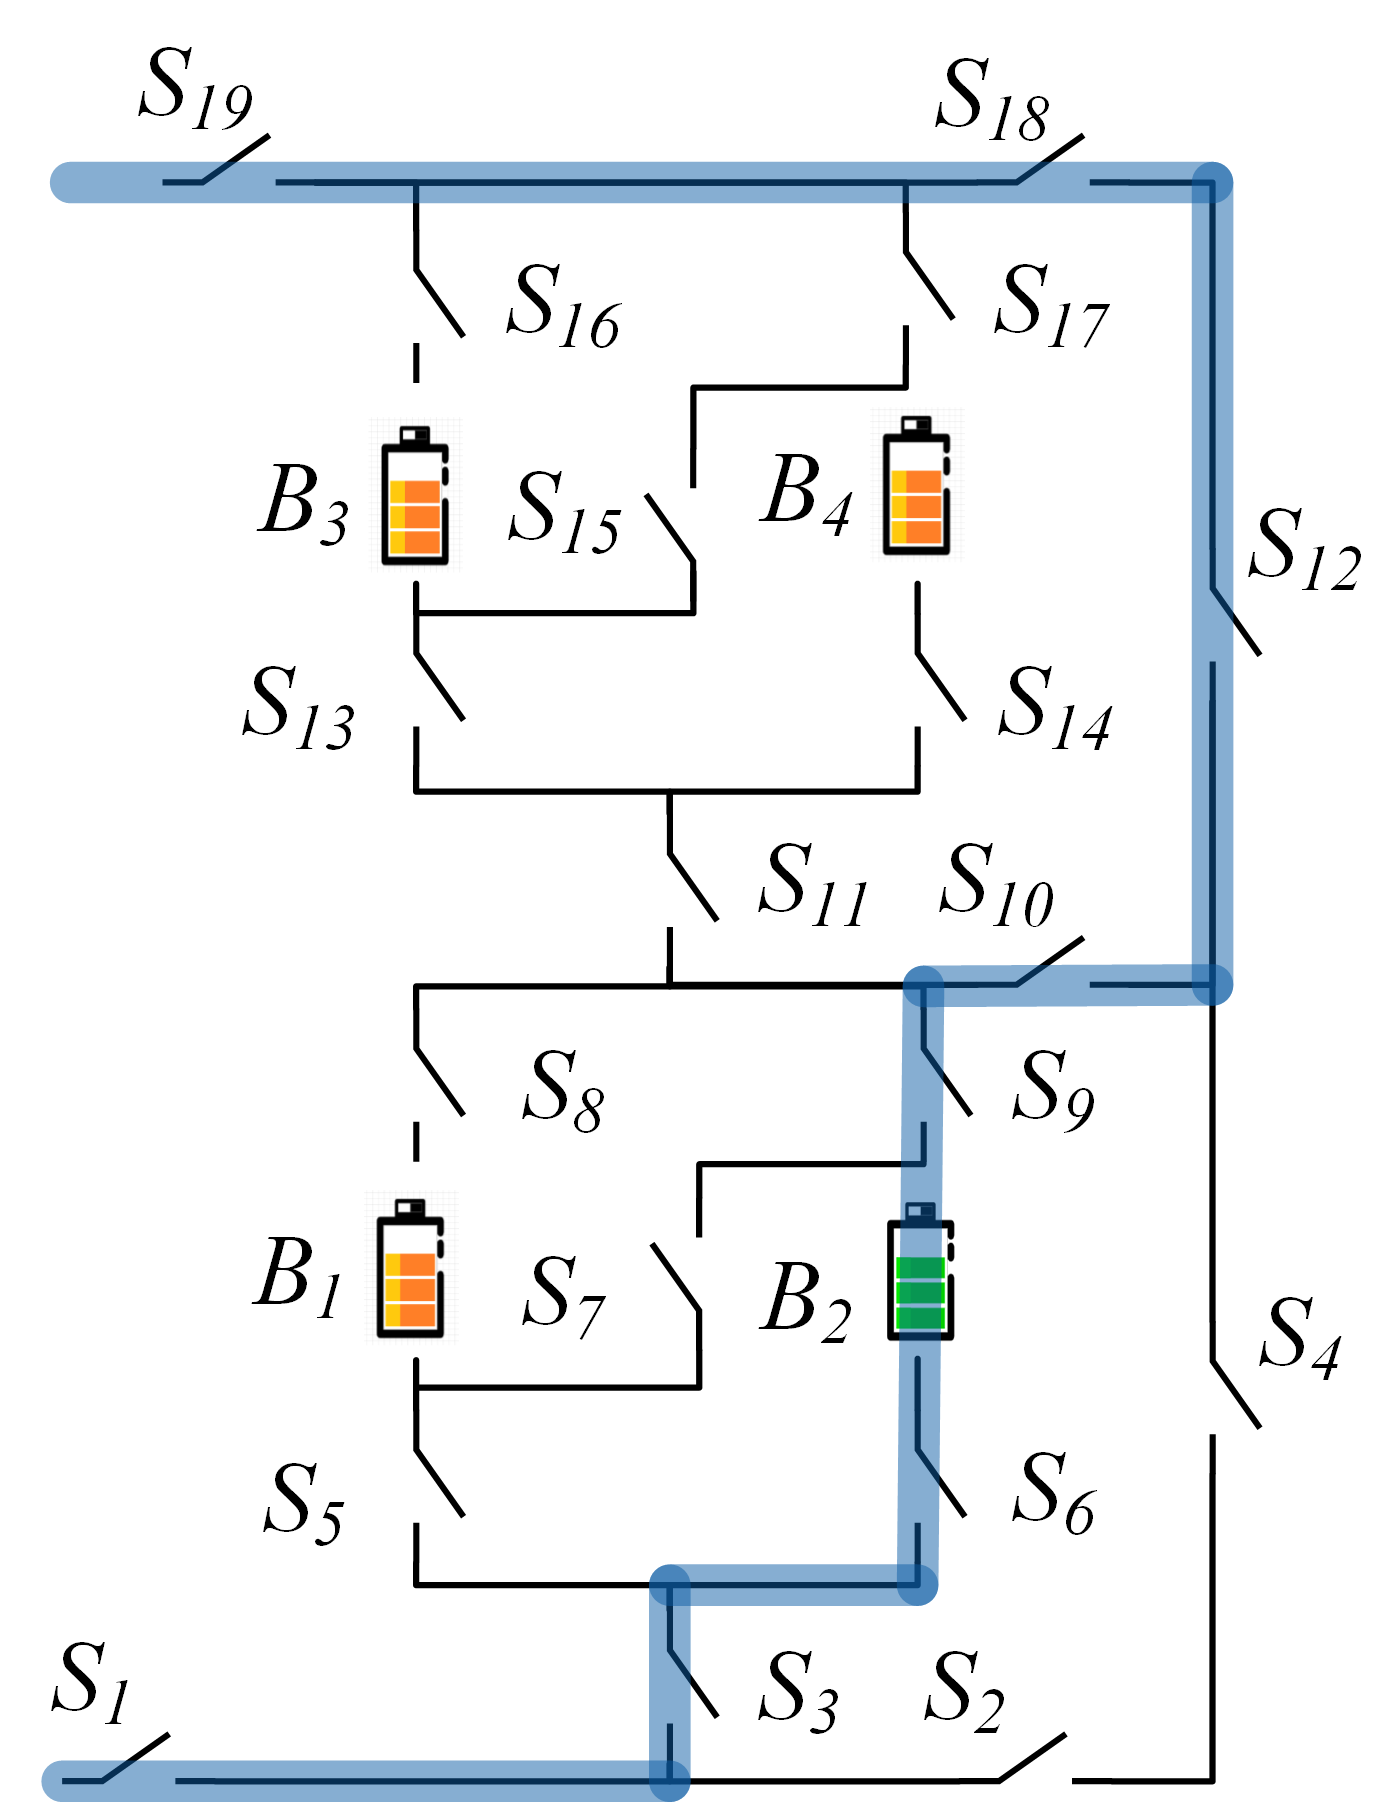
\includegraphics[width=\textwidth]{e2f2-isolate-3.png}
        \caption{}
        \label{fig:my-isolated-3}
    \end{subfigure}
    \caption{
        Circuit states of MACs when isolating (a) one, (b) two (in different substructures), (c) two (in the same substructure), and (d) three batteries for the structure in Fig. \ref{fig:study-stru-my}.
        }
\end{figure}

\subsection{Discussion}

\subsubsection{correctness of the results}

The correctness of the outcomes provided by the proposed greedy algorithm will be discussed from two perspectives: circuit analysis and validation against the brute-force algorithm. 
Let's take the four-battery RBS structure shown in Fig. \ref{fig:study-stru-my} as an example.
When $B_1$ and $B_2$ or $B_3$ and $B_4$ are connected in parallel, the RBS produces the maximum current, which is $\eta=2$ (i.e., twice the current output of a single battery in the RBS). 
Adding more batteries to the main circuit only creates a series structure and does not improve the MAC. 
Therefore, the switch-control scheme provided in Tab. \ref{tab:study-results-my} maximizes the RBS output current.
On the other hand, the brute-force method, which examines all possible switch states, also yields the same $\eta$.
This indicates that the proposed greedy algorithm successfully identifies the MAC among all the potential reconfigured structures.

\subsubsection{advantages and disadvantages of our method}

The proposed greedy algorithm possesses a significant advantage in terms of its effectiveness and efficiency. 
In this paper, it is compared with the brute-force algorithm, SA, and GA. 
While the brute-force algorithm ensures the correctness of the results by exploring all possible switch states, it comes at a high computational cost. 
The SA and GA are commonly used heuristic algorithms for addressing NP-hard problems. 
They selectively generate solutions for the switching states to maximize the objective value $\eta$.
However, neither of these two algorithms can determine whether the current $\eta$ represents the final MAC or if they should continue searching for better solutions. 
Moreover, as depicted in Figs. \ref{fig:e4-alg}--\ref{fig:e2f2-alg} and Figs. \ref{fig:e2f1-alg}--\ref{fig:e2f3-alg}, the SA and GA algorithms require more iterations to converge to the final solution compared to the proposed greedy algorithm. 
In contrast, the proposed greedy algorithm can identify the correct MAC in a shorter number of steps.


To further elaborate on the efficiency of our algorithm, we analyze the time complexity of both the brute-force algorithm and the greedy algorithm.
If an RBS has $N_b$ batteries and $N_s$ switches and the corresponding directed graph has $N$ nodes,  $2^{N_s}$ iterations are required to traverse all reconfigured structures.
Calculating each reconfigured structure using Eqs. (\ref{eq:I_o})--(\ref{eq:eta}) requires matrix inversion and matrix multiplication, which has a time complexity of $O(N^3+2N^2N_b+N^2N_s+NN^2_b)$.
Therefore, the time complexity of the brute-force algorithm is $O\bm((N^3+2N^2N_b+N^2N_s+NN^2_b)2^{N_s}\bm)$.
The greedy algorithm proposed in this paper requires  that SP be found for each battery, which requires $N_b$ iterations.
Each SP can be obtained by several applications of Dijkstra's algorithms.
Therefore, the total time complexity for calculating all SPs is $O\bm(N_b(N_b+2N_s)\log_{10} N\bm)$.
According to  Appendix \ref{alg:greedy}, the RBS can reconfigure $C^{N_{\text{set}}}_{N_b}$ structures by selecting $N_{\text{set}}$ batteries from $N_b$ batteries, which gives $\sum^{N_b}_{N_{\text{set}}=1}C^{N_{\text{set}}}_{N_b}/N_b \approx 2^{N_b} N_b^{-1}$ on average.
Thus, with the bisection method, the time complexity of the greedy algorithm is $O\bm((N^3+2N^2N_b+N^2N_s+NN^2_b) 2^{N_b} N_b^{-1} \log_{10} N_b+N_b(N_b+2N_s)\log_{10} N\bm)$.
Based on currently proposed RBS structures \cite{ciNovelDesignAdaptive2007,alahmadBatterySwitchArray2008,kimDependableEfficientScalable2010b,kimBalancedReconfigurationStorage2011a,taesickimSeriesconnectedSelfreconfigurableMulticell2012a,6843711}, the number $N_b$ of batteries, $N_s$ of switches, and $N$ of nodes are quantitatively related as follows: $N_s \approx (3\text{--} 5)N_b$, $N \approx N_s$. 
After simplifying, the time complexity of the method with greedy algorithm is $O(2^{N_b}N_s^2\log_{10} N_b)$, while it is $O(2^{N_s}N_s^3)$ for the method with brute-force algorithm.
Therefore, as the RBS grows, especially in the number of switches, the greedy algorithm gains an advantage over the brute-force algorithm.
This is confirmed by the number of structures required to determine the MAC in the previous section. 
Compared with the brute-force algorithm, the method based on the greedy algorithm is 3\,000 to 48\,000 times more efficient, which is theoretically $N_s 2^{N_s - N_b} \log_{10} N_b$ times according to the above time-complexity analysis.
This benefits from two key points:
\begin{enumerate}
    \item[(1)] The SPs guide the RBS to reconfigure reasonable structures rather than blindly going through all possible structures. This reduces the complexity from $2^{N_s}$ to $2^{N_b}$, which is the main reason for the improvement in efficiency. 
    \item[(2)] The bisection method further accelerates this process, reducing the complexity from $2^{N_b}$ to $2^{N_b} N_B^{-1} \log_{10} N_b$.
\end{enumerate}


Furthermore, this approach has the capability to handle RBSs with arbitrary structures, which is another significant advantage of it. 
It is able to correctly calculate the MACs of RBSs with arbitrary structures, even when they have different variant batteries, or even random isolated batteries. 
Theoretically, each RBS structure can be transformed into the unique directed graph model using the methodology described in the Section II, and the MAC can subsequently be calculated using the proposed greedy algorithm.
This finding has been supported in the previous subsection. 


However, the suggested greedy algorithm still includes exponential terms in its time complexity, indicating that it struggles to perform at scale. 
Additionally, all batteries are assumed to be identical for the sake of simplification in the derivation.
However, there may exist a small balancing current, which could introduce a minor bias to the MAC, due to variations in open-circuit voltage $u_b$ and internal resistance $r_b$ in reality.
Nevertheless, the proposed greedy algorithm remains a viable choice for the RBS design and optimization in the early stage, and the issue of balancing current bias can be addressed by considering the variations in batteries and replacing the internal resistance with impedance when constructing the directed graph model.

\subsubsection{application scenarios}

Note that $\eta$ is used as the objective function instead of $I_o$ in solving for the MAC. 
This choice makes the resulting MAC more reasonable and applicable in practical scenarios. 
As shown in Tab. \ref{tab:study-results-my}, $I_o$ and $\bm{I}_b$ are functions of $R_o$, $u_b$, and $r_b$. 
However, when $I_o$ is used as the objective function, even for the same RBS structure, the MAC solution and corresponding switch states could change due to different external electrical appliances.
This would increase the difficulty and uncertainty of designing the RBS structure. 
To eliminate this problem, the ratio $\eta=I_o/\max(\bm{I}_b)$ is adopted as the objective function in our research.
Recall that $\eta$ reflects only the structure's ability to output current, rather than the actual current outputing by the battery system.
Assuming that the MAC of batteries in the RBS is $I_m$, the maximum output current of the RBS structure can be calculated as $\eta I_m$ by determining the value of $\eta$ for the structure. 


The method proposed in this paper facilitates the design of RBSs in the following ways:
most currently proposed RBS structures \cite{ciNovelDesignAdaptive2007,alahmadBatterySwitchArray2008,kimDependableEfficientScalable2010b,kimBalancedReconfigurationStorage2011a,taesickimSeriesconnectedSelfreconfigurableMulticell2012a,6843711} have simple topological characteristics, so calculating the MACs is relatively straightforward, even intuitive.
However, these simple structures do not always fully satisfy the requirements of complex applications, such as dynamically adapting the circuit to variable and random operating conditions or actively equalizing differences between batteries in the RBS.
Moreover, isolating the batteries disrupts the original regularity and symmetry of the topology, which complicates the otherwise simple structure, and the maximum output current of the system becomes more challenging to obtain.
In contrast, the proposed method calculates the MAC of arbitrary RBS structures, notably the complex and flexible RBS structures.


To illustrate this point, the MACs of the RBS structure in Fig. \ref{fig:study-stru-my} are calculated after isolating one or more of the batteries, as shown in Figs. \ref{fig:my-isolated-1}--\ref{fig:my-isolated-3}. 
When a single battery is isolated, the RBS is still capable of outputting the maximum current, denoted as $\eta=2$.
When two batteries are isolated, there are two scenarios: 
one is isolating two batteries within the same substructure (Figure \ref{fig:my-isolated-2b}), resulting in $\eta=2$; the other is isolating one battery in each of the two substructures (Figure \ref{fig:my-isolated-2w}), resulting in $\eta=1$. 
If three batteries are isolated, the RBS can only output the current of a single battery, which is $\eta=1$.
Therefore, the battery management system can adjust the output current and control the RBS to reconfigure the corresponding structure based on the isolated batteries.


\section{Conclusion}

This paper proposes a pervasive and automated method to efficiently compute the MAC of an RBS.
The method is implemented by a greedy algorithm combined with an improved directed graph model.
Not only does the method provides the same global MAC calculation results as the brute-force method, but it also demonstrates superior computational efficiency compared to both the brute-force algorithm and the heuristic algorithms (SA and GA). 
Theoretically, for an RBS with $N_s$ switches and $N_b$ batteries, the efficiency of the proposed method is $N_s 2^{N_s - N_b} \log_{10} N_b$ times that of the brute-force method. 
This is primarily due to the utilization of the batteries' SPs to guide the RBS to reconfigure reasonable structures rather than blindly going through all possible structures.
Another advantage of this method is its capability to calculate the MAC of RBSs with arbitrary structures and variant batteries. 
Even in scenarios with random isolated batteries, the proposed method remains effective.
This method facilitates the full utilization of the RBS's current output potential, guides the design and optimization of the RBS structure during the design stage, and assists in evaluating the risk of current overload in practical applications.

\section{Appendix} 

\begin{algorithm}
    \caption{Get the max available currents of a certain RBS}\label{alg:greedy}
    \KwData{Directed graph model $G(V,E)$ of the RBS}
    \KwResult{$\max \eta$}
    \For{$i \in E_b$}{
        $P_i \leftarrow \{path| \text{starts at $v_1$ and ends at $v_n$} \}$\;
        $SP_i \leftarrow p_i \text{ which has the minimum}~\omega(p_i)~\text{among all}~p_i \in P_i. $
    }
    get $\bm{A}$ by Eq. \ref{eq:A}\;
    \While{not yet determine $\max \eta$ }
    {
        $N_{\text{set}} \leftarrow$ number of setected SPs calculated by dichotomy\;
        $C_b    \leftarrow$ set of all combinations of $N_{\text{set}} $~batteries from $N_b$\;
        \For{$c_b \in C_b$}{
            $\bm{x}_s \leftarrow \text{list of all switches' state: $x_s[j]=1$ if $ j \in \bigcup_{i\in c_b}SP_i $ else 0}$\;
            $\bm{X} \leftarrow diag[1,1,\cdots,1,\bm{x}_s] $\;
            get $\bm{Y}_n$ by Eq. \ref{eq:Yn}\;
            \eIf{$\bm{Y}_n$ is invertible}{
              pass
            }{construct an effective solution}
            get $I_o$ by Eq. \ref{eq:I_o}\;
            get $\bm{I}_b$ by Eq. \ref{eq:I_b}\;
            \eIf{$\max(\bm{I}_b)\leq I_m$}{
                $\eta \leftarrow I_o/\max(\bm{I}_b)$\;
            }{break}
        }
    }
\end{algorithm}
% \begin{figure}[htbp]
%     \centering
%     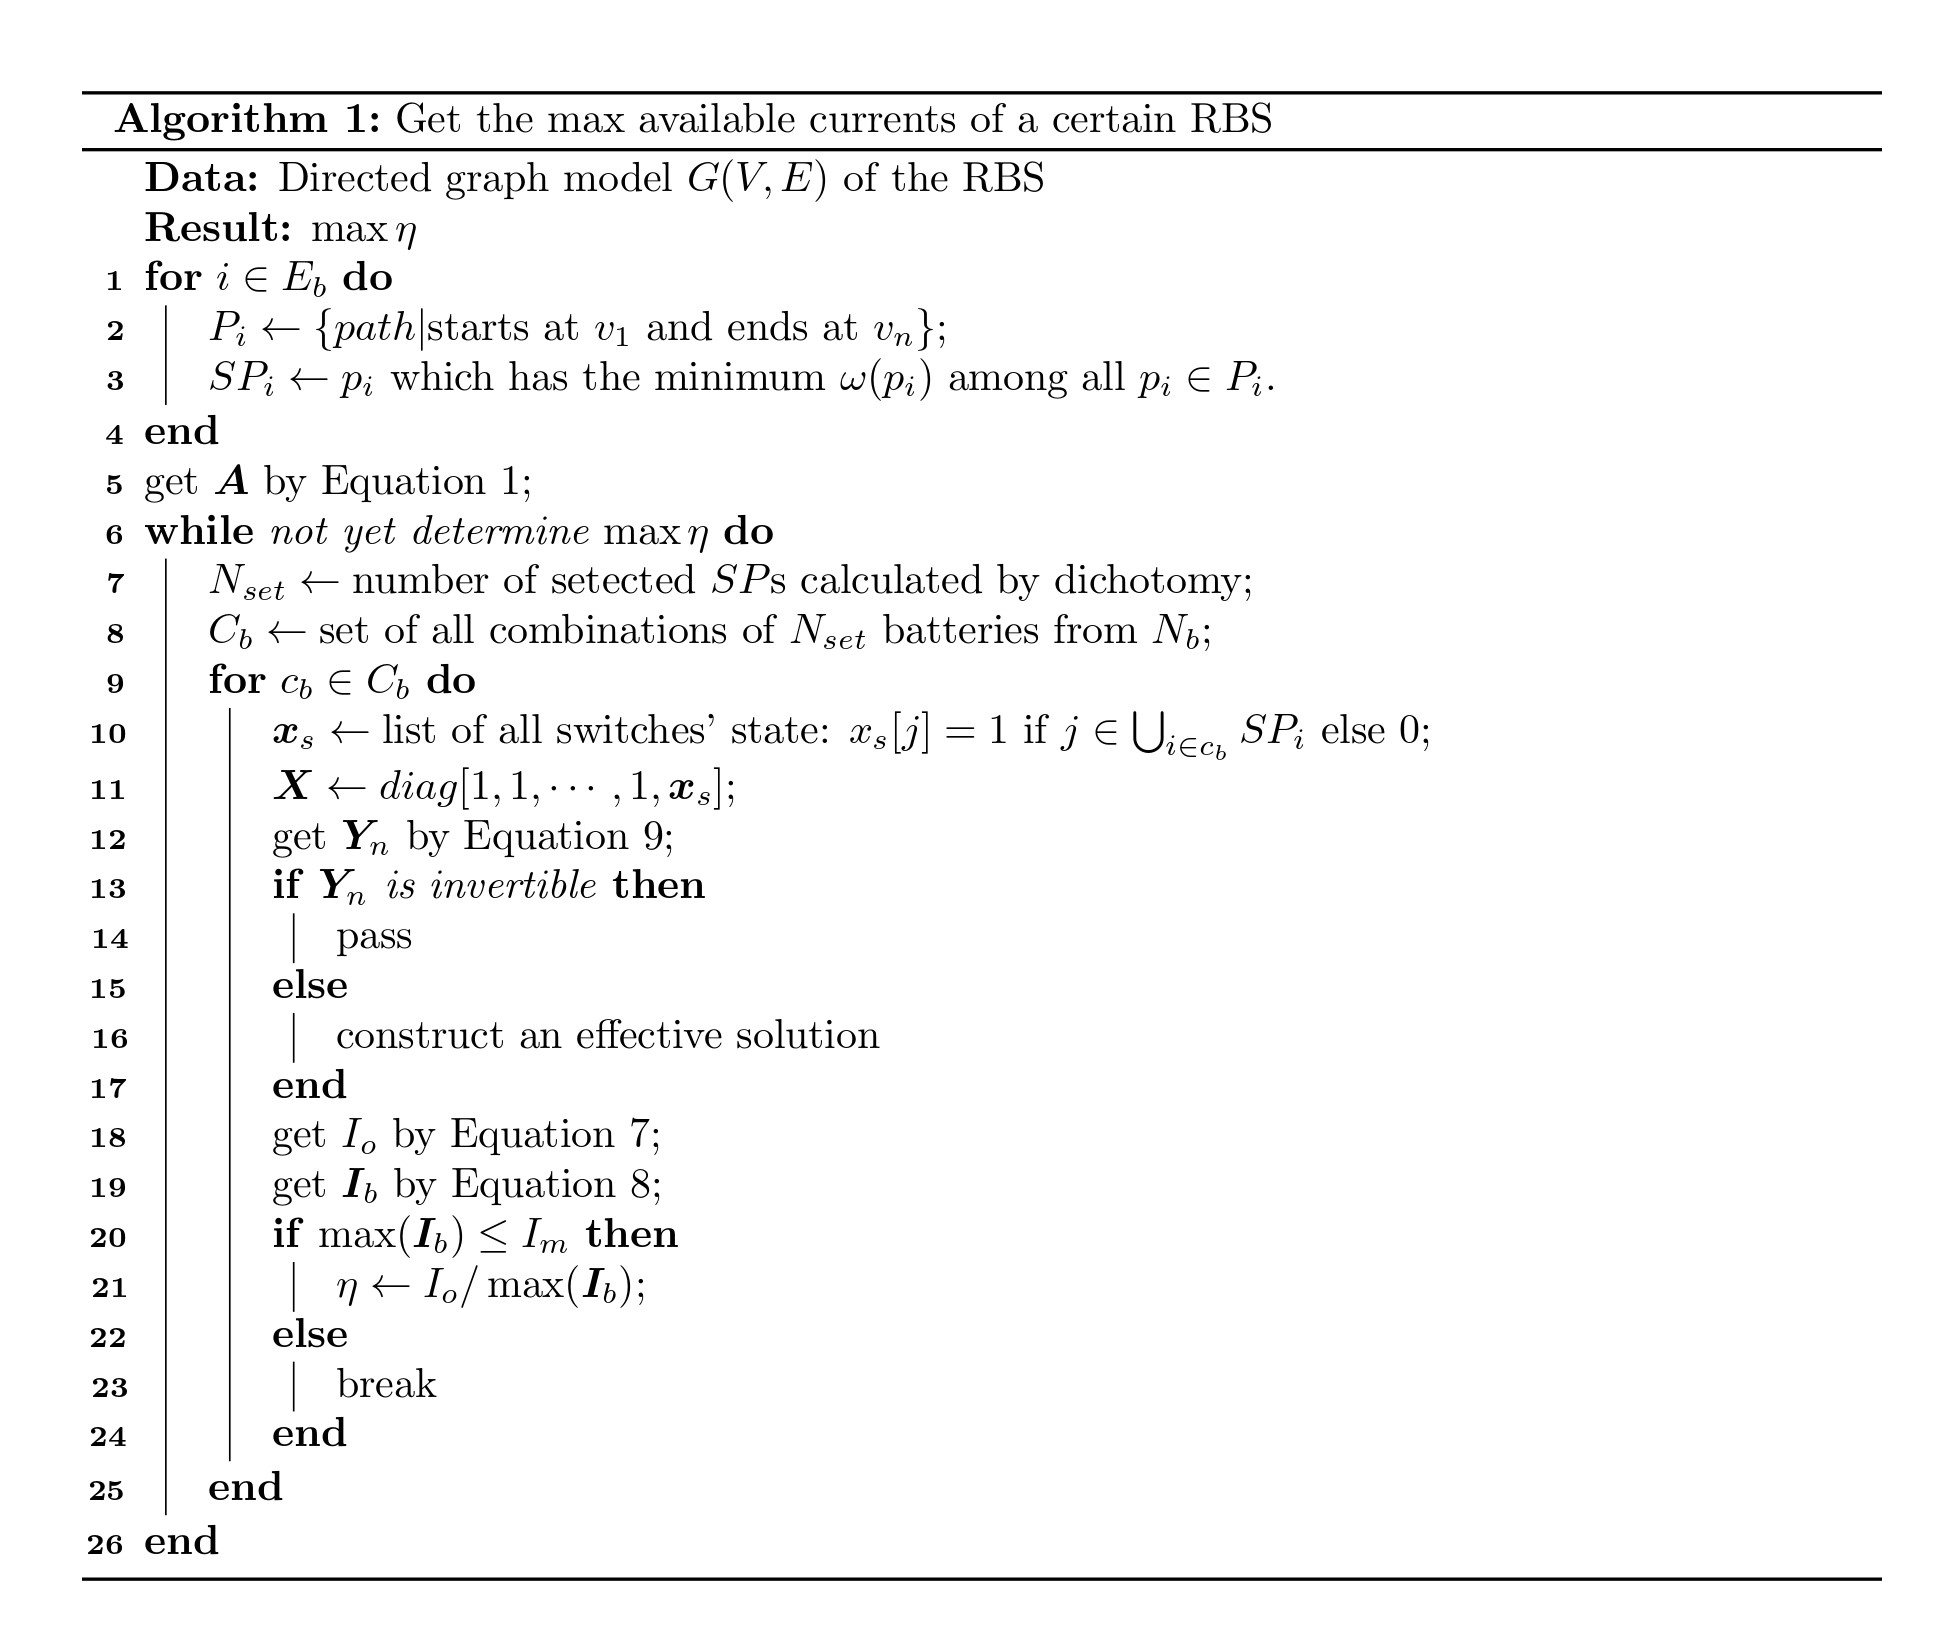
\includegraphics[width=\textwidth]{algorithm.jpg}
% \end{figure}


\section*{Acknowledgments}

\subsection*{Author Contributions} 

B. Xu conceived the main idea, formulated the overarching research goals and aims, designed the algorithm, and reviewed and revised the manuscript.
G. Hua developed and analyzed the model, implemented the code and supporting algorithms, and wrote the initial draft.
C. Qian provided critical review, commentary, and revisions.
Q. Xia contributed to shaping the research, analysis, and manuscript.
B. Sun conducted the research and investigation process.
Y. Ren secured the funding and supervised the project.
Z. Wang verified the results and provided necessary resources.

% \subsection*{Funding}
% 
% This work was supported by the National Natural Science Foundation of China (NSFC, No.52075028).

\subsection*{Conflicts of Interest}

The authors declare that there is no conflict of interest regarding the publication of this article.

\subsection*{Data Availability}

This work does not require any data to be declared or publicly disclosed.

\bibliographystyle{unsrt}
\bibliography{ref}

% \begin{thebibliography}{10}
% 
% \bibitem{yangBatteryEnergyStorage2018}
% Yuqing Yang, Stephen Bremner, Chris Menictas, and Merlinde Kay.
% \newblock Battery energy storage system size determination in renewable energy systems: {{A}} review.
% \newblock {\em Renewable and Sustainable Energy Reviews}, 91:109--125, August 2018.
% 
% \bibitem{desiqueiraControlStrategySmooth2021}
% Luanna Maria~Silva {de Siqueira} and Wei Peng.
% \newblock Control strategy to smooth wind power output using battery energy storage system: {{A}} review.
% \newblock {\em Journal of Energy Storage}, 35:102252, March 2021.
% 
% \bibitem{schwanbeckInternationalSpaceStation2019}
% Eugene Schwanbeck and Penni Dalton.
% \newblock International {{Space Station Lithium-ion Batteries}} for {{Primary Electric Power System}}.
% \newblock In {\em 2019 {{European Space Power Conference}} ({{ESPC}})}, pages 1--1. {IEEE}, September 2019.
% 
% \bibitem{zhangDevelopmentProspectChinese2021}
% Lihua Zhang.
% \newblock Development and {{Prospect}} of {{Chinese Lunar Relay Communication Satellite}}.
% \newblock {\em Space: Science \& Technology}, 2021, January 2021.
% 
% \bibitem{choCommercialResearchBattery2015}
% Jaephil Cho, Sookyung Jeong, and Youngsik Kim.
% \newblock Commercial and research battery technologies for electrical energy storage applications.
% \newblock {\em Progress in Energy and Combustion Science}, 48:84--101, June 2015.
% 
% \bibitem{yangUnbalancedDischargingAging2016}
% Naixing Yang, Xiongwen Zhang, BinBin Shang, and Guojun Li.
% \newblock Unbalanced discharging and aging due to temperature differences among the cells in a lithium-ion battery pack with parallel combination.
% \newblock {\em Journal of Power Sources}, 306:733--741, February 2016.
% 
% \bibitem{fengPropagationMechanismsDiagnosis2019}
% Fei Feng, Xiaosong Hu, Lin Hu, Fengling Hu, Yang Li, and Lei Zhang.
% \newblock Propagation mechanisms and diagnosis of parameter inconsistency within {{Li-Ion}} battery packs.
% \newblock {\em Renewable and Sustainable Energy Reviews}, 112:102--113, September 2019.
% 
% \bibitem{jeevarajanBatterySafetyQualifications2012}
% J.~A. Jeevarajan and C.~Winchester.
% \newblock Battery {{Safety Qualifications}} for {{Human Ratings}}.
% \newblock {\em Interface magazine}, 21(2):51--55, January 2012.
% 
% \bibitem{pomboHybridPowerSystem2021}
% Daniel~V{\'a}zquez Pombo.
% \newblock A {{Hybrid Power System}} for a {{Permanent Colony}} on {{Mars}}.
% \newblock {\em Space: Science \& Technology}, 2021, January 2021.
% 
% \bibitem{hanNextGenerationBatteryManagement2020a}
% Weiji Han, Torsten Wik, Anton Kersten, Guangzhong Dong, and Changfu Zou.
% \newblock Next-{{Generation Battery Management Systems}}: {{Dynamic Reconfiguration}}.
% \newblock {\em IEEE Industrial Electronics Magazine}, 14(4):20--31, December 2020.
% 
% \bibitem{visairoReconfigurableBatteryPack2008}
% H.~Visairo and P.~Kumar.
% \newblock A reconfigurable battery pack for improving power conversion efficiency in portable devices.
% \newblock In {\em 2008 7th {{International Caribbean Conference}} on {{Devices}}, {{Circuits}} and {{Systems}}}, pages 1--6. {IEEE}, April 2008.
% 
% \bibitem{ci2007novel}
% Song Ci, Jiucai Zhang, Hamid Sharif, and Mahmoud Alahmad.
% \newblock A novel design of adaptive reconfigurable multicell battery for power-aware embedded networked sensing systems.
% \newblock In {\em IEEE GLOBECOM 2007-IEEE Global Telecommunications Conference}, pages 1043--1047. IEEE, 2007.
% 
% \bibitem{9209774}
% Jan Engelhardt, Tatiana Gabderakhmanova, Gunnar Rohde, and Mattia Marinelli.
% \newblock Reconfigurable stationary battery with adaptive cell switching for electric vehicle fast-charging.
% \newblock In {\em 2020 55th International Universities Power Engineering Conference (UPEC)}, pages 1--6, 2020.
% 
% \bibitem{engelhardt2021double}
% Jan Engelhardt, Jan~Martin Zepter, Tatiana Gabderakhmanova, Gunnar Rohde, and Mattia Marinelli.
% \newblock Double-string battery system with reconfigurable cell topology operated as a fast charging station for electric vehicles.
% \newblock {\em Energies}, 14(9):2414, 2021.
% 
% \bibitem{lawsonSoftwareConfigurableBattery2012}
% Barrie Lawson.
% \newblock A {{Software Configurable Battery}}.
% \newblock {\em EVS26 International Battery, Hybrid and Fuel Cell Electric Vehicle Symposium}, 2012.
% 
% \bibitem{he2014reconfiguration}
% Liang He, Linghe Kong, Siyu Lin, Shaodong Ying, Yu~Gu, Tian He, and Cong Liu.
% \newblock Reconfiguration-assisted charging in large-scale lithium-ion battery systems.
% \newblock In {\em 2014 ACM/IEEE International Conference on Cyber-Physical Systems (ICCPS)}, pages 60--71. IEEE, 2014.
% 
% \bibitem{kim2009dynamic}
% Hahnsang Kim and Kang~G Shin.
% \newblock On dynamic reconfiguration of a large-scale battery system.
% \newblock In {\em 2009 15th IEEE Real-Time and Embedded Technology and Applications Symposium}, pages 87--96. IEEE, 2009.
% 
% \bibitem{han2021analysis}
% Weiji Han, Anton Kersten, Changfu Zou, Torsten Wik, Xiaoliang Huang, and Guangzhong Dong.
% \newblock Analysis and estimation of the maximum switch current during battery system reconfiguration.
% \newblock {\em IEEE Transactions on Industrial Electronics}, 69(6):5931--5941, 2021.
% 
% \bibitem{chenSneakCircuitTheory2021}
% Si-Zhe Chen, Yule Wang, Guidong Zhang, Le~Chang, and Yun Zhang.
% \newblock Sneak {{Circuit Theory Based Approach}} to {{Avoiding Short-Circuit Paths}} in {{Reconfigurable Battery Systems}}.
% \newblock {\em IEEE Transactions on Industrial Electronics}, 68(12):12353--12363, 2021.
% 
% \bibitem{heExploringAdaptiveReconfiguration2013}
% Liang He, Lipeng Gu, Linghe Kong, Yu~Gu, Cong Liu, and Tian He.
% \newblock Exploring {{Adaptive Reconfiguration}} to {{Optimize Energy Efficiency}} in {{Large-Scale Battery Systems}}.
% \newblock In {\em 2013 {{IEEE}} 34th {{Real-Time Systems Symposium}}}, pages 118--127, December 2013.
% 
% \bibitem{hongwenheStateofChargeEstimationLithiumIon2011}
% Hongwen He, Rui Xiong, Xiaowei Zhang, Fengchun Sun, and JinXin Fan.
% \newblock State-of-{{Charge Estimation}} of the {{Lithium-Ion Battery Using}} an {{Adaptive Extended Kalman Filter Based}} on an {{Improved Thevenin Model}}.
% \newblock {\em IEEE Transactions on Vehicular Technology}, 60(4):1461--1469, May 2011.
% 
% \bibitem{mousavig.VariousBatteryModels2014}
% S.M. Mousavi~G. and M.~Nikdel.
% \newblock Various battery models for various simulation studies and applications.
% \newblock {\em Renewable and Sustainable Energy Reviews}, 32:477--485, April 2014.
% 
% \bibitem{ciNovelDesignAdaptive2007}
% Song Ci, Jiucai Zhang, Hamid Sharif, and Mahmoud Alahmad.
% \newblock A {{Novel Design}} of {{Adaptive Reconfigurable Multicell Battery}} for {{Power-Aware Embedded Networked Sensing Systems}}.
% \newblock In {\em {{IEEE GLOBECOM}} 2007-2007 {{IEEE Global Telecommunications Conference}}}, pages 1043--1047, November 2007.
% 
% \bibitem{alahmadBatterySwitchArray2008}
% Mahmoud Alahmad, Herb Hess, Mohammad Mojarradi, William West, and Jay Whitacre.
% \newblock Battery switch array system with application for {{JPL}}'s rechargeable micro-scale batteries.
% \newblock {\em Journal of Power Sources}, 177(2):566--578, March 2008.
% 
% \bibitem{kimDependableEfficientScalable2010b}
% Hahnsang Kim and Kang~G. Shin.
% \newblock Dependable, efficient, scalable architecture for management of large-scale batteries.
% \newblock In {\em Proceedings of the 1st {{ACM}}/{{IEEE International Conference}} on {{Cyber-Physical Systems}}}, {{ICCPS}} '10, pages 178--187, {New York, NY, USA}, April 2010. {Association for Computing Machinery}.
% 
% \bibitem{kimBalancedReconfigurationStorage2011a}
% Younghyun Kim, Sangyoung Park, Yanzhi Wang, Qing Xie, Naehyuck Chang, Massimo Poncino, and Massoud Pedram.
% \newblock Balanced reconfiguration of storage banks in a hybrid electrical energy storage system.
% \newblock In {\em 2011 {{IEEE}}/{{ACM International Conference}} on {{Computer-Aided Design}} ({{ICCAD}})}, pages 624--631, November 2011.
% 
% \bibitem{taesickimSeriesconnectedSelfreconfigurableMulticell2012a}
% Taesic Kim, Wei Qiao, and Liyan Qu.
% \newblock A series-connected self-reconfigurable multicell battery capable of safe and effective charging/discharging and balancing operations.
% \newblock In {\em 2012 {{Twenty-Seventh Annual IEEE Applied Power Electronics Conference}} and {{Exposition}} ({{APEC}})}, pages 2259--2264, February 2012.
% 
% \bibitem{6843711}
% Liang He, Linghe Kong, Siyu Lin, Shaodong Ying, Yu~Gu, Tian He, and Cong Liu.
% \newblock Reconfiguration-assisted charging in large-scale {{Lithium-ion}} battery systems.
% \newblock In {\em 2014 {{ACM}}/{{IEEE International Conference}} on {{Cyber-Physical Systems}} ({{ICCPS}})}, pages 60--71, April 2014.
% 
% \end{thebibliography}

% \printbibliography

\end{document}
